%%%%%%%%%%%%%%%%%%%%%%%%%%%%%%%%%%%%%%%%%%%%%%%%%%%%%%%%%%%%%%%%%%%%%%%%%%%%%%%
% M.Sc. Libre Software URJC 2012
%
% Report for Project Evaluation subject
% Laura Arjona Reina (larjona99@gmail.com)
% Cesar Valiente Gordo (cesar.valiente@gmail.com)
% Esther Parrilla-Endrino (eparrillae@gmail.com)
%
%%%%%%%%%%%%%%%%%%%%%%%%%%%%%%%%%%%%%%%%%%%%%%%%%%%%%%%%%%%%%%%%%%%%%%%%%%%%%%%

\documentclass[a4paper,10pt]{article} 
\usepackage[utf8]{inputenc}
\usepackage[english]{babel}
\usepackage[hyphens]{url}
\usepackage[colorlinks=true,linkcolor=black,urlcolor=black,bookmarksopen,
breaklinks]{hyperref}
%\usepackage{breakurl}
%%%%%%%%%%%%%%%%%%%%%%%%%%%%%%%%%%%%%%%%%%%%%%%%%%%%%%%%%%%%%%%%
%% ccBeamer 0.1, 2007-07-02                                   %%
%% Written by Sebastian Pipping <webmaster@hartwork.org>      %%
%% ---------------------------------------------------------- %%
%% Licensed under Creative Commons Attribution-ShareAlike 3.0 %%
%% http://creativecommons.org/licenses/by-sa/3.0/             %%
%%%%%%%%%%%%%%%%%%%%%%%%%%%%%%%%%%%%%%%%%%%%%%%%%%%%%%%%%%%%%%%%


%% Images
\newcommand{\CcImageBy}[1]{%
	
\includegraphics[scale=#1]{creative_commons/cc_by_30.pdf}%
}
\newcommand{\CcImageCc}[1]{%
	
\includegraphics[scale=#1]{creative_commons/cc_cc_30.pdf}%
}
\newcommand{\CcImageDevNations}[1]{%
	
\includegraphics[scale=#1]{creative_commons/cc_dev_nations_30.pdf}%
}
\newcommand{\CcImageNc}[1]{%
	
\includegraphics[scale=#1]{creative_commons/cc_nc_30.pdf}%
}
\newcommand{\CcImageNd}[1]{%
	
\includegraphics[scale=#1]{creative_commons/cc_nd_30.pdf}%
}
\newcommand{\CcImagePd}[1]{%
	
\includegraphics[scale=#1]{creative_commons/cc_pd_30.pdf}%
}
\newcommand{\CcImageSa}[1]{%
	
\includegraphics[scale=#1]{creative_commons/cc_sa_30.pdf}%
}
\newcommand{\CcImageSampling}[1]{%
	
\includegraphics[scale=#1]{creative_commons/cc_sampling_30.pdf}%
}
\newcommand{\CcImageSamplingPlus}[1]{%
	
\includegraphics[scale=#1]{creative_commons/cc_sampling_plus_30.pdf}%
}


%% Groups
\newcommand{\CcGroupBy}[1]{% zoom
	\CcImageBy{#1}%
}
\newcommand{\CcGroupByNc}[2]{% zoom, gap
	\CcImageBy{#1}\hspace*{#2}\CcImageNc{#1}%
}
\newcommand{\CcGroupByNcNd}[2]{% zoom, gap
	\CcImageBy{#1}\hspace*{#2}\CcImageNc{#1}\hspace*{#2}\CcImageNd{#1}%
}
\newcommand{\CcGroupByNcSa}[2]{% zoom, gap
	\CcImageBy{#1}\hspace*{#2}\CcImageNc{#1}\hspace*{#2}\CcImageSa{#1}%
}
\newcommand{\CcGroupByNd}[2]{% zoom, gap
	\CcImageBy{#1}\hspace*{#2}\CcImageNd{#1}%
}
\newcommand{\CcGroupBySa}[2]{% zoom, gap
	\CcImageBy{#1}\hspace*{#2}\CcImageSa{#1}%
}
\newcommand{\CcGroupDevNations}[1]{% zoom
	\CcImageDevNations{#1}%
}
\newcommand{\CcGroupNcSampling}[2]{% zoom, gap
	\CcImageNc{#1}\hspace*{#2}\CcImageSampling{#1}%
}
\newcommand{\CcGroupPd}[1]{% zoom
	\CcImagePd{#1}%
}
\newcommand{\CcGroupSampling}[1]{% zoom
	\CcImageSampling{#1}%
}
\newcommand{\CcGroupSamplingPlus}[1]{% zoom
	\CcImageSamplingPlus{#1}%
}


%% Text
\newcommand{\CcLongnameBy}{Attribution}
\newcommand{\CcLongnameByNc}{Attribution-NonCommercial}
\newcommand{\CcLongnameByNcNd}{Attribution-NoDerivs}
\newcommand{\CcLongnameByNcSa}{Attribution-NonCommercial-ShareAlike}
\newcommand{\CcLongnameByNd}{Attribution-NoDerivs}
\newcommand{\CcLongnameBySa}{Attribution-ShareAlike}

\newcommand{\CcNote}[1]{% longname
	This work is licensed under the \textit{Creative Commons #1 3.0 License}.%
}

\usepackage{amssymb}
\usepackage{eurosym}
\usepackage{verbatim}
\usepackage{fancyhdr} 
\usepackage{amsmath}
\usepackage{graphicx}
\usepackage{pdfpages}
\usepackage{float}
\usepackage{caption3} 
\DeclareCaptionOption{parskip}[]{} 
\usepackage[small]{caption}
\usepackage{latexsym}  %% For additional characters
\usepackage{rotating}
\usepackage[table]{xcolor}

\title {Evaluation of SCM systems:\\ SVN, Git and Mercurial}
\author{Laura Arjona Reina (larjona99@gmail.com)\\Cesar Valiente Gordo
(cesar.valiente@gmail.com)\\Esther Parrilla-Endrino (eparrillae@gmail.com)\\
 M.Sc. Libre Software URJC}
\date{\today}

\begin{document}
\sloppy
\maketitle

\newpage
\thispagestyle{empty}
\vspace{5cm}
\begin{flushright}
\begin{large}
Copyright \copyright 2011 Laura Arjona Reina,\\ Cesar Valiente Gordo,\\ Esther
Parrilla-Endrino.\\
Some Rights Reserved.\\
This work is licensed under the\\
Creative Commons Attribution 3.0 License.\\
To view a copy of this license, visit\\
\url{http://creativecommons.org/licenses/by/3.0/}\\
or send a letter to\\
Creative Commons,\\
543 Howard Street, 5th Floor, San Francisco,\\
California, 94105, USA.\\
\end{large}
\end{flushright}
\vspace{13cm}
\begin{center}
\CcGroupBy{1.20}\\
{\tiny\CcNote{\CcLongnameBy}}
\end{center}

\newpage
\tableofcontents
\newpage
\renewcommand{\refname}{Bibliography}
\addtolength{\parskip}{\baselineskip}

%%%%%%%%%%%%%%%%%%%%%%%%%%%%%%%%%%%%%%%%%%%%%%%%%%%%%%%%%%%%%%%%%%%%%
\section{Introduction}
The main goal of this trade-off analysis is to recommend a suitable SCM
(software configuration management) system for
start-up called \textbf{Amiguetes S.L.}, to install in their own infrastructure
(personal PCs, servers) and hold the development projects of the company.

\subsection{Context Information}
\subsubsection{Overview}

For a better understanding on how the trade-off analysis of the different SCMs
was performed it is necessary first to know some context information about the
people who started this analysis and their environment.

At the beginning of this year (2011) and due to the complex situation in the
Spanish labor market, five friends decided to join efforts and begin a small
start-up company called \textbf{Amiguetes S.L.} that may bring new professional
opportunities to them.

The idea is to take advantage of the professional experience that each of them
have in the Software development field, specially implementing Open Source
solutions.

As currently the market of mobile applications is very active and
Android\cite{Android} is the leading solution (according to the latest
studies\cite{Smartphone}) they decide to focus their business model in producing
high-level add-ons to improve the functionalities of Android-based smartphones
and tablets.

One detail to take into account is that these friends live in different parts of
Spain, so they will work in a distributed way and not everyone will have the
same role and dedication to the project, three of them (the most experienced)
will be part of the ``Core" of the developers layer (according to the ``Onion
Model"\cite{Onion}) taking the responsibility of implementing moreless the 70\%
of the code and fully dedicated to the project; and the other two will be part
of the ``Co-developers" layer, with just part-time dedication.

Also the idea is to incorporate external contributors (the ``Active Users"
layer) from past projects, FLOSS communities interested in mobile applications
development, friends etc.

To be able to coordinate the contributions of such heterogeneous group of
developers they realize that it is going to be mandatory to use a SCM\cite{SCM}
system and from the existing FLOSS solutions they decide to perform a trade-off
analysis of the following ones: Subversion\cite{Subversion}, Git\cite{Git} and
Mercurial\cite{Mercurial}, this document is the result of that comparison.

Some of the ``core'' developers have experience using CVS\cite{CVS} so they
would
prefer to move to a more similar system like Subversion but others have heard
about distributed SCMs and think it would better to try those kind of solutions
(Git or Mercurial) due to the distributed nature of the project's contributors.

\subsubsection{Interactions}
Which SCM to use is an important decision, but source code management is only a
part of a software company's infrastructure, and setting how this component
interacts with others will uncover some aspects that should be desirable to be
found in the used SCM.
\begin{itemize}
\item To facilitate the involvement of new developers in the community, the
"core developers" have the idea of setting up a common development environment
that any commiter can setup locally and start contributing as soon as possible
to the project, for that reason, it should be desirable that our SCM has:
 \begin{itemize}
  \item Easy installer in most used desktop OS (Windows, Linux, MacOS), packaged
bundles (.rpm, .deb etc...) will be preferable but also it should be possible
to install the repository from sources.
  \item Repository GUI clients, that make easier the management of code for
those developers who are not very familiar with command-line clients and instead
prefer to operate with the repository graphically.
  \item As part of the common development environment setup, the core developers
have already selected Eclipse as the development default IDE because it provides
a dedicated Android plugin\cite{AndroidPlugin} that boosts implementation
process. It would be good also to be able to integrate the SCM version
management system into Eclipse so all the code management process gets unified
in a single tool.
 \end{itemize}
\item To increase the visibility of the company repository, it would be useful
if it is web browseable. This may be faced in two ways: whether the SCM provides
a web browser interface, or the repository can be accessed in some way from the
company's website, written in Drupal\cite{Drupal} (for example, by a Drupal
module to view repositories).
\item The core developers want to try to bring new contributors to their
community, therefore it would be nice if there are existing plugins to integrate
the repositories with software forges, specially with bug tracking systems. They
must decide in which public forge they prefer to host their developments,
possible options they are evaluating include: Google Code\cite{GoogleCode},
Launchpad\cite{Launchpad}, Sourceforge\cite{Sourceforge} or Github\cite{Github}.
\item To give more value to the SCM which they need to chose, the group
of friends were wondering it would be good if the SCM could be integrated in a
\textit{virtual machine} like \textbf{VMWare}\footnote{http://www.vmware.com/}
or \textbf{VirtualBox}\footnote{https://www.virtualbox.org/}.
As we said before, at the beginning they want to use a forge which could be
integrate the appropriate SCM, but thinking in the future maybe to expand their
business and buying their own machines this question is really interesting.
\item Would be interesting to know if the SCM could have any system to make
automatic backups in an easy way, could be an integrated system, a plug-in to add to the SCM, or using conventional scripts.
\end{itemize}
\subsubsection{List of requirements}
Here we list the above mentioned requirements, grouped in categories:
\begin{itemize}
 \item Functionality: web browseable, distributed, with plugins for Eclipse and
forges integration. Virtual machine integration, integration with backup
systems.
 \item Usability: easy to use or similar to CVS, easy installer, GUI
clients.
 \item Adoption: widely used tool (easy that new developers know it)
 \item Community: live and smart community, according with the desired image
for a startup company.
 \item Documentation and support: easy to learn, not required to spend time in
solving problems.
\end{itemize}

\subsection{Research goals}
These are the main goals of this research:
\begin{itemize}
\item Analyze the different SCM in order to know if they match our requirements
(yes/no; degree)
\item Provide a comparative report showing metrics explaining the appropriate
degree to these requirements, following an standardized process.
\item State in the report other important features of each SCM, to take into
account despite of not being considered initially as requirements.
\item Recommend the tool that best matches the company's requirements.
\item Explain the weak points of the chosen tool, to take into account.
\item Provide references on the data sources, methodology and process followed,
in order to make this study reproducible.
\end{itemize}

%%%%%%%%%%%%%%%%%%%%%%%%%%%%%%%%%%%%%%%%%%%%%%%%%%%%%%%%%%%%%%%%%%%%%
\section{Methodology}

\subsection{Data sources}
\label{datasources}
For analyzing the different software configuration management systems and
provide a reliable comparison, data from different sources will be used. In
this section we present the most important ones; other sources will be
referenced or explained directly (for example using a footnote) when the
corresponding fact, metric or argument is discussed.

\subsubsection{Existing work}
\label{Existingwork}
Some of the members of Amiguetes S.L., had carried a previous research about
this topic and fulfilled some OpenBRR sheets with metrics about Git, Subversion
and Mercurial. We will analyze that existing work and take it as an initial
point. 

The original templates of the previous research and evaluation of SCMs, made by
the students of Master on Libre Software of Universidad Rey Juan Carlos
(Madrid, Spain) in 2011, may be downloaded from:

Git: \url{
https://gitorious.org/mswl-eval/mswl-eval/blobs/master/ProjectEvaluation_Report/
OpenBRR_Templates/BRR_Template_Git_mswl.ods}


Mercurial: \url{
https://gitorious.org/mswl-eval/mswl-eval/blobs/master/ProjectEvaluation_Report/
OpenBRR_Templates/BRR_Template_Mercurial_mswl.ods}


Subversion: \url{
https://gitorious.org/mswl-eval/mswl-eval/blobs/master/ProjectEvaluation_Report/
OpenBRR_Templates/BRR_Template_SVN_mswl.ods}

For more information about this topic you can visit the MSWL Project Evaluation
Subject's Moodle site in
\url{http://docencia.etsit.urjc.es/moodle/course/view.php?id=125}.

\subsubsection{Official websites}
The official websites of the SCMs provide reliable information about their
functionality, history, documentation and support. These sites are listed below:
\begin{itemize}
 \item Subversion: \url{http://subversion.apache.org}
 \item Git: \url{http://git-scm.com/}
 \item Mercurial: \url{http://mercurial.selenic.com}
\end{itemize}

\subsubsection{Other data sources}
Ohloh metrics will be taken into account. Ohloh\cite{Ohloh} is a free public
directory of open source software and people, owned and operated by BlackDuck
Software Inc., a consulting company specialized in gathering and providing
information about open source software projects. Some metrics present in Ohloh
site are provided by Ohloh specific tools and others are provided by gathering
the information provided by Ohloh users for their own projects or the projects
they are interested in.

In addition to this, some metrics will be calculated directly inspecting the
source code and history of the development of the different SCMs (that is, their
own commit logs). For this task, FLOSSMetrics databases will be used.
FLOSSMetrics\cite{FLOSSMetrics} stands for Free/Libre Open Source Software
Metrics, and it is an European Commission founded project with the goal to
(among
others) publish a large scale database with information and metrics about libre
software development. The dumps for Git, SVN and Mercurial contain data about
the development of each project until November 22nd, 2011.

\subsection{Type of approach: OpenBRR}
The Business Readiness Rating model (OpenBRR)\cite{OpenBRRWhitepaper} is
intended to help IT managers
assess which Open Source software would be most suitable for their needs. Open
Source users can also share their evaluation ratings with potential adopters,
continuing the virtuous cycle and “architecture of participation” of open
source.

The initiative is lead by the Carnegie Mellon West University, Spike Source,
Intel and O’Reilly’s Code Zoo and offer proposals for standardizing different
types of evaluation data and grouping them into categories.

The framework suggests the following metrics to be analyzed and evaluated:
\begin{itemize}
\item Functionality
\item Usability
\item Quality
\item Security
\item Performance
\item Scalability
\item Architecture
\item Support
\item Documentation
\item Adoption
\item Community
\item Professionalism
\end{itemize}

The model is composed of the following phases:
\begin{itemize}
\item Phase 1 - Quick Assessment: defining and ranking of metrics and categories
according to their importance within the product that is going to be evaluated.
\item Phase 2 - Target usage assessment: Set the necessary category and metric
weights according to the project's goals.
\item Phase 3 - Data collection and processing: Gather data for each metric used
in each category rating, and calculate the applied weighting for each metric,
spreadsheets are used for this purpose.
\item Phase 4 - Data translation: Use category ratings and the functional
orientation weighting factors to calculate the Business Readiness Rating score
and publish the software’s Business Readiness Rating score.
\end{itemize}

The Business Readiness Rating model offers a trusted and open framework for
software evaluation, this model aims to accelerate the software evaluation
process with a systematic approach, facilitate the exchange of information
between IT managers, result in better decisions, and increase confidence in
high-quality open source software.

\subsection{OpenBRR improvements with new metrics}
\label{OpenBRRimprovements}
Some OpenBRR requirements are evaluated with poor metrics. We are going to
decide some more metrics to improve this evaluations.
\subsubsection{Developers taking care of documentation}
\label{NewMetricLarjona1}
A new metric is introduced in the \textbf{Documentation} category. This
category is measured in the original OpenBRR model with the existence of
detailed documentation about the software, and the existence of user-to-user
help. We also think that it is very important that while the software evolves,
developers care about documentation updates. So we are going to introduce a new
metric consisting in counting the number of commits with the word
``documentation'' in their log message. To normalize the metric we will
divide the obtained sum by the total number of commits. The score assigned to
this metrics will be:
\begin{itemize}
 \item Less than 1\% of total commits: 1
 \item Between 1\% and 5\% of total commits: 3
 \item More than 5\% of total commits: 5
\end{itemize}

\subsubsection{Distance between the two most active authors}
\label{NewMetricLarjona2}
A new metric is introduced in the \textbf{Community} category, consisting in
measure the balance between the effort of the two most active authors of the
project.

To calculate the metric we will divide the number of commits of each developer
by the sum of the commits performed by the two of them, obtaining a percentage
of the effort of the two more active developers. The raw score would be the
difference between the two efforts.

We believe that depending too much on the main developer is a weakness for the a
software developer community, since this individual may abandon the project and
would be difficult to find a new leader. If most of the contributions are
balanced between two persons, the weakness of depending on a certain individual
would be less. On the other side, we need to take in account also the danger of
having "two leaders" in a project: differences between them or disagreements in
project roadmaps may lead to forks and damage the sustainability of the
community. The same occurs when "no leader" can be clearly found: a project may
lack of clear roadmap or nobody would assume responsibilities.

So the normalized scores to assign to this metric will be:
\begin{itemize}
 \item More than 50\%, or less than 10\%: 1
 \item Between 20\% and 30\%: 5
 \item Other: 3
\end{itemize}

\subsubsection{Longevity}
\label{NewMetricEparrillae1}
A new metric is introduced in the \textbf{Community} category. This category is measured in the original OpenBRR model with the "Average volume of general mailing list in the last 6 months" and the "Number of unique code contributors in the last 6 months". 

We think that the longevity of a given project must be measured combining two
different criteria, in one hand the project's age, for example Subversion is
more than ten years old and still alive which is a good point for that SCM. But
apart from that, also it has to be analyzed if during the whole project
lifecycle there has been development activity, a very old project with just a
few activity is really useless for us :-)

Taking into account the previous assertions the normalized scores to assign to this metric will be:
\begin{itemize}
 \item Young project (more than 1 year old) and increasing lines of code production : 1
  \item Medium project (more than 5 years old) and increasing lines of code production : 3
 \item Long project (more than 10 years old) and increasing lines of code production: 5
\end{itemize}

\subsubsection{License}
\label{NewMetricEparrillae2}

A new metric is introduced in the \textbf{Professionalism} category. This category is measured in the original OpenBRR model with "Project Driver" and "Difficulty to enter the core developer team".

We think it is a positive point that the SCM is licensed under an OSI-approved\footnote{http://www.opensource.org/licenses} FLOSS license. Also if the license allows to mix the product with proprietary code is an enhancement.

Taking into account the previous assertions the normalized scores to assign to this metric will be:
\begin{itemize}
 \item Open Source but Non-OSI-Approved license: 1
 \item OSI-Approved and "GPL-like" license: 3
 \item OSI-Approved and "weak copyleft" license: 5
\end{itemize}

\subsubsection{Programming Languages} \label{Programming Languages}

This new metric is introduced in the \textbf{Architecture} category since we
think is really important the way the SCM is building.

For us is important to give to new developers the possibility to be involved in
a FLOSS project, if the project is completely building based in just one
programming language is possible that a developer who doesn't know about the
language used on it, can't collaborate in a FLOSS project which is really
interesting for him, in the other side, if the project uses more programming
languages is easier new developers can participate on it.

But also is important the amount of code used in a concrete programming
language, wouldn't be good if we say that a FLOSS project uses three different
programming languages when one of them just has 100 lines of code.

To give a rating to value this new metric we are going to follow the next rules:
\begin{itemize}
 \item 80\% or more written in one language: 1
 \item 80\% or more written in two languages: 3
 \item 80\% or more written in three or more languages: 5
\end{itemize}

\subsubsection{Contributors} \label{Contributors2}

This new metric is introduced in the \textbf{Community} category since we
think is really important the way developers collaborate in the projects.

FLOSS projects are based in two different ways to collaborate, the
\textit{cathedral} and \textit{the bazaar}, the first has very few group of
developers who develop the entire application, the second one is based in much
more collaboration from much more developers.

We prefer this last one option, we think is much more convenient and healthy
for a FLOSS project if the effort is distributed as much as it can be possible,
but we know that is really difficult because despite having projects with big
amount of developers, a very important number of commits are done by the same
developers following the \textit{onion skin model}, so we are going to follow
the next model to value this metric:

\begin{itemize}
 \item 40\% or more developed by less than 3 developers: 1
 \item 40\% or more developed between 3 to 7 developers: 3
 \item 40\% or more developed by more to 7 developers: 5 
\end{itemize}

\section{Analysis and Results}

\subsection{OpenBRR application}
\label{OpenBRR_application}
We are going to follow the ``Business Readiness Rating for Open Source
(OpenBRR)'' whitepaper\cite{OpenBRRWhitepaper} to apply this model to the
evaluation of the software configuration managements Git, Mercurial and
Subversion.

\subsubsection{Phase 1: Quick Assessment}
This first phase has been already applied before our analysis, and three SCM
passed it to further evaluation: Git, Mercurial and Subversion.
\subsubsection{Phase 2: Target Usage Assessment}
This second phase consists in, as explained before, setting the category and
metric weights according to the company's requirements. The canonical OpenBRR
model recommends to focus in not more than seven categories, but in order to
provide a more general overview, we will consider the twelve categories present
in the model.

If we were considering all the categories equal in importance, we should weight
each one of them with 8,33\%. Our assessment will consider this number, in
order to weight more than 8\% the categories considered relevant for the
company, and less than 8\% the categories considered not so relevant for the
company.

The most important selected categories have been \textbf{functionality},
\textbf{usability} and \textbf{community}. Each one of them have been given a
weight of 12\%, so together they reach 36\% of the total evaluation.


The OpenBRR model provides no ready-to-collect metrics for
\textbf{functionality}, allowing the evaluator to create them in a tailored way
according to the customer's requirements. This is an opportunity for us to
measure here specific requirements as support for distributed environments and
local repositories (important for Amiguetes S.L.) or support for branches, tags,
diffs and merges (specific for SCM functionality). Other desirable functionality
metrics for the SCM used in Amiguetes S.L. would be the existence of
internationalization and multi-platform support, since the company wants to
lower the access barrier to new developers, despite the language they speak or
the operating system they use.


About \textbf{usability}, we already stated that Amiguetes S.L. need a SCM easy
to learn so the developers may not invest too much time in infrastructure tasks
and focus on developing software for Android.


The existence of an active \textbf{community} is also important for Amiguetes
S.L.: it would be a marketing failure to choose an old, near-to-death or
latter abandoned SCM for a young, starting company (plus the costs of migration
to a new SCM if the currently used is being abandoned by their
[formers] developers and active users.


\textbf{Support} and \textbf{documentation} are also desirable aspects, that
ensure the liveness of the community of any piece of software, and also
guarantee usability since good instructions and advices smooth out the
difficulties of any tool. For this reasons this two categories have been
weighted with 10\%. With the same arguments we could consider
\textbf{adoption}, but we also need to know that there are two influent factors
in adoption: on one hand, we need time for any tool to be widely used, so a
young SCM not very popular now, may in the future be the most used. On the
other hand, ``trends'' have also influence in the IT world; and certain
companies or tools come in a particular time to the crest of the wave, but
quickly sink into obscurity due to the dynamism of the technologies
environments. So adoption have been scored with 9\%, still over the mean, but
not so much.


About \textbf{security}, the given weight has been 8\%, since Amiguetes S.L.
has no particular requirements about this aspect, but it is a desirable feature
specially for the future when new developers come to the community.


Performance and architecture are two categories weighted under the mean (6\%).
\textbf{Performance} is always good, but Amiguetes S.L. is a starting company
and the intended pieces of software to develop are small widgets or
applications, so it is not so important if there is a small lack of performance
because the small projects would not suffer it. About \textbf{architecture}, it
is true that some requirements have been mentioned about plugins to integrate
the SCM with the Eclipse IDE and with software forges, but we consider those
requirement very specific and it would be no good if a certain SCM have a very
good architecture or many plugins but not the ones that we need.


The less important categories for this evaluation are \textbf{quality},
\textbf{scalability} and \textbf{professionalism}. These categories have been
weighted with 5\%, which makes a sum of 15\% of total evaluation. This low
weight does not mean that Amiguetes S.L. does not care about these aspects, but
that the three evaluated SCM already provide high scores for these categories
and the small differences between them are not so determinant to choose one or
the other. 


In conclusion, in table \ref{OpenBRR2} we can present here the categories and
their resulting weights for our evaluation.

\begin{table}[ht]
\begin{center}
    \begin{tabular}{ | l | c | r |}
    \hline
    \textbf{Rank} & \textbf{Category} & \textbf{Weight} \\ \hline
    1 & Functionality & 12\% \\ \hline
    2 & Usability & 12\% \\ \hline
    3 & Quality & 5\% \\ \hline
    4 & Security & 8\% \\ \hline
    5 & Performance & 6\% \\ \hline
    6 & Scalability & 5\% \\ \hline
    7 & Architecture & 6\% \\ \hline
    8 & Support & 10\% \\ \hline
    9 & Documentation & 10\% \\ \hline
    10 & Adoption & 9\% \\ \hline
    11 & Community & 12\% \\ \hline
    12 & Professionalism & 5\% \\ \hline
     & \textbf{TOTAL WEIGHT} & \textbf{100\%} \\ \hline  
    \end{tabular}
\end{center}
 \caption{OpenBRR Target Usage Assessment for SCM to be used in Amiguetes S.L.}
\label{OpenBRR2}
\end{table}

\subsubsection{Phase 3: Data collection and processing}
The team have used the OpenBRR framework with a spreadsheet provided by the
students of Master on Libre Software (Universidad Rey Juan Carlos, Madrid,
Spain), as commented in section \ref{Existingwork}. This spreadsheet has an
initial set of metrics for each OpenBRR category, allowing to ponderate each
metric and providing a normalized score according to the possible values
obtained in measurements.
To the existing set of features, 6 more metrics have been added to the
corresponding categories, in order to materialize the OpenBRR improvements
explained in section \ref{OpenBRRimprovements}.
Category weights have been introduced in the sheets. Each metric within each
category should have a weighting factor to differentiate the metric's
importance withing that particular category. For simplicity, we have
distributed equally the different weights when the particular set of metrics
was not relevant according to the company's requirements, and followed a
similar process as in phase 2 (target usage assessment) when the measured
aspects were particularly relevant to the company's requirements.
As a result, we have a new blank OpenBRR spreadsheet to use as template for the
data collection and processing. This spreadsheet can be downloaded from:

\url{
https://gitorious.org/mswl-eval/mswl-eval/blobs/master/ProjectEvaluation_Report/
OpenBRR_Templates/BRR_Template_amiguetes.ods}

Each metric has been measured using one of the following methods:
\begin{itemize}
 \item Trusting the metric score and reference provided by previous research
(mswl templates) mentioned in section \ref{Existingwork}.
 \item Measuring ourselves the aspect or category using the data sources
mentioned in section \ref{datasources}.
 \item Searching the Internet and getting the needed information from official
mailing lists or websites (and referencing that link in the corresponding ``Raw
score'' cell with a ``comment'' in the cell.
\end{itemize}

In most of the cases you can find a reference from were we obtained the metric
by inspecting the ``Raw score'' cells (showing the cell comments). When a
reference is not provided, it means that that metric could not be found
or the own tool command line help or main website announces that aspect so it is
easy to find.

For the unknown data, we have assigned the worst possible normalized score to
the corresponding metric, so the results is not biased by unreliable
information.

\subsubsection{Phase 4: Representative Metrics and their Scoring}

After collecting all the data and normalizing using the OpenBRR spreadsheet,
scores for each category and a global score is automatically calculated.
The resulting work can be downloaded from this URLs:
\begin{itemize}
 \item Git OpenBRR spreadsheet:
\url{
https://gitorious.org/mswl-eval/mswl-eval/blobs/master/ProjectEvaluation_Report/
OpenBRR_Templates/BRR_Template_Git_larjona_final.ods}

 \item Mercurial OpenBRR spreadsheet:
\url{
https://gitorious.org/mswl-eval/mswl-eval/blobs/master/ProjectEvaluation_Report/
OpenBRR_Templates/BRR_Template_Mercurial_cvaliente_final.ods}

 \item Subversion OpenBRR spreadsheet:
\url{
https://gitorious.org/mswl-eval/mswl-eval/blobs/master/ProjectEvaluation_Report/
OpenBRR_Templates/BRR_Template_SVN_eparrillae_final.ods}

\end{itemize}

The total results for each SCM are: Subversion 3.2215, Git 3.774, Mercurial
3.66. The SCM obtaining a better score is \textbf{Git}, being the one
recommended to be used in Amiguetes S.L.

After analyzing Subversion we have reached the conclusion that although this SCM
is quite stable and reliable and very easy to use its centralized design it is
becoming a bit obsolete nowadays therefore it does not seem to be a good option
for a start-up company like Amiguetes S.L. The company may need in the future
certain functionalities that are not currently present in SVN and as the planned
releases are not so frequent as in the other solutions it may take a bit longer
until the tool is updated, also the fact that not all the most popular FLOSS
forges provide support for SVN is a big disadvantage for this option as the
company has in mind trying to move their code in the future to a public forge to
try to join more contributors to its community, for that reason we discard SVN
as a valid solution for Amiguetes S.L.

Once SVN is discarded, we had to choose between the other two distributed solutions Git or Mercurial, the main weaknesses for Mercurial compared to Git is the fact that it is not as known as Git and do not have behind such a huge community like the Linux Kernel development team. Also in the analysis of the contributors distribution we have seen that if one of the key "core developers" leave Mercurial that could be problematic, this something that has to be taken into account by Amiguetes S.L.

\subsection{Recommended tool}

Git\cite{Git} is a cross-platform, distributed Open Source Software
Configuration Management (SCM), focused in speed and high performance.

Current version is 1.7.8, released in December 2nd, 2011
\footnote{\url{http://article.gmane.org/gmane.linux.kernel/1223707}}, licensed
under the terms of \textbf{GNU GPLv2}.

Among its main features we can mention that allows distributed development
(local copies of the entire development history),support for different
protocols, fast branching and merging, Unix-like toolkit design. There are
multiple pieces of software, developed by the Git community an others, to
integrate this SCM with other tools and extend its functionality.

\subsubsection{Deployment}

People of Amiguetes S.L. should read carefully the Appendix about Git to begin
to learn the tool, specially from where to download, where are the main
websites to obtain help and documentation for quickly learn to use the tool.

It would be nice if they create and maintain a wiki in their website dedicated
to new developers, explaining the steps that they are following to learn an use
the tool: the problems that newcomers to Amiguetes S.L. community face to use
git for contributing may be similar to the problems that Amiguetes S.L.'s
developer faced when they began to use the tool.

They can install git-core and later add some of its plugins or tools to get
the integration that they wanted: eGit plugin to use with Eclipse, gitweb to
offer their repositories as web browseable if they host a mirror of the
repository in their webserver.

They can host their repositories in many software forges. If they decide to use
GitHub, they can use certain references when committing to link GitHub issue
tracker with git.

They can visit the page
\url{https://git.wiki.kernel.org/articles/i/n/t/Interfaces,_frontends,
_and_tools.html} to learn more about tools to integrate git with backups,
continous integration systems, and other things they need. 

They can use Agit application (\url{https://github.com/rtyley/agit}) to interact
with their git repositories from their tablets and other Android devices.

They should set some rules about how to name branches and other type of
git usage. The Note from the Git
Maintainer\footnote{\url{
http://git-blame.blogspot.com/p/note-from-maintainer.html } } may be a good
guide since git developers know very well how git works and how to take the
best from it and use it in an elegant way.

Android source code is also developed using Git. This is an advantage: it
would be easy for Amiguetes S.L. to integrate in the Android community since
they use the same tools. The Android Open Source web pages about version
control (\url{http://source.android.com/source/version-control.html}) may also
be very useful for them, since they can act as a good reference or guide to set
the Git policy of Amiguetes S.L. 

\section{Conclusions and further work}

\subsection{Lessons learnt in this exercise}

In this report we have learnt to evaluate three different SCMs following one of the evaluation methodologies we have seen in the "Project Evaluation" subject of the Master, the OpenBRR methodology.

We have to say that we believe this methodology covers most of the main aspects of a given project in terms of functionality, usability, scalability etc... so we think it is a very good way to start evaluating a given solution.

But while evaluating the metrics we saw that there were some analysis aspects
that were out of the scope of OpenBRR templates done in the class and it was
necessary to introduce new metrics to complete the report, specially we think
the templates failed to provide a "community oriented" point of view, for that
reason most of the metrics we have introduced are in the "Community" category.

In any case, this exercise provides a very valuable way to perform trade-off analysis of certain FLOSS products and the fact of having templates that automate the calculation of the overall score for each solution is really useful.

\subsection{Reproducibility instructions}
This study may be reproduced at any time with updated data, or little changes
to adapt the OpenBRR model to different requirements. 

To update the evaluation with new data, the steps to follow are:
\begin{itemize}
 \item Obtain the new dumps from FLOSSMetrics or directly clone the
repositories and pass LibreSoft CVSanaly tool to them.
\item Create a database for each repository and dump the FLOSSMetrics data or
the CVSanaly SQL data to it.
\item Recalculate each metric by visiting the link present in each cell's
comment, or following the steps mentioned in the corresponding section of this
document.
\item For measuring Functionality category, follow the OpenBRR
Whitepaper\cite{OpenBRRWhitepaper}.
\end{itemize}

If you just need to add a new SCM to the pool of projects evaluated, you can
download a copy the ``blank template'' (tailored weights and functionality
category) from here:

 \url{
https://gitorious.org/mswl-eval/mswl-eval/blobs/master/ProjectEvaluation_Report/
OpenBRR_Templates/BRR_Template_amiguetes.ods}

Then you rename your copy to use it with the data of the new SCM, and fulfill
the spreadsheet with the corresponding data (similar steps as updating the
study with new data, explained before).


If the requirements change, it will be necessary to rewrite all the
weights of OpenBRR categories and metrics, in order to match the new
requirements. You can follow a similar process as has been done before (section
\ref{OpenBRR_application}).

\subsection{About this study}
\subsubsection{People involved, resources invested}
This trade-off analysis has been implemented by the following people of the MSWL:

\begin{itemize}
\item Cesar Valiente Gordo (cesar.valiente@gmail.com).
\item Esther Parrilla-Endrino (eparrillae@gmail.com).
\item Laura Arjona Reina (larjona99@gmail.com).
\end{itemize}

We have done this report using Gitorius as collaborative tool, the repository created by Laura can be found in the following location:

\url{https://gitorious.org/mswl-eval}

All work performed is licensed under the Creative Commons Attribution 3.0 License\footnote{http://creativecommons.org/licenses/by/3.0/}.

All sections of this report have been implemented by the three of us, with the exception of the specific SCM appendix that have been implemented by:

\begin{itemize}
\item SVN: Esther Parrilla-Endrino.
\item Git: Laura Arjona Reina.
\item Mercurial: Cesar Valiente Gordo.
\end{itemize}

About the new metrics introduced for OpenBRR improvements, each one of us write
two new metrics:
\begin{itemize}
\item Laura Arjona Reina designed metric ``Developers taking care of
documentation'' (explained in section \ref{NewMetricLarjona1} and integrated in
the customized OpenBRR spreadsheet for Amiguetes S.L., category
``Documentation''\cite{OpenBRR_amiguetes}), and metric ``Distance between the
two most active authors'' (explained in section \ref{NewMetricLarjona2} and
integrated in the customized OpenBRR spreadsheet for Amiguetes S.L., category
``Community''\cite{OpenBRR_amiguetes}).

\item Esther Parrilla-Endrino designed metric Longevity (explained in section
\ref{NewMetricEparrillae1} and integrated in
the customized OpenBRR spreadsheet for Amiguetes S.L., category
``Community''\cite{OpenBRR_amiguetes}), and metric ``License'' (explained in section
\ref{NewMetricEparrillae2} and
integrated in the customized OpenBRR spreadsheet for Amiguetes S.L., category
``Professionalism''\cite{OpenBRR_amiguetes}).
\item Cesar Valiente Gordo designed metric Programming Languages (explained in section
\ref{Programming Languages} and integrated in
the customized OpenBRR spreadsheet for Amiguetes S.L., category
``Architecture''\cite{OpenBRR_amiguetes}), and metric ``Contributors'' (explained in section
\ref{Contributors2} and
integrated in the customized OpenBRR spreadsheet for Amiguetes S.L., category
``Community''\cite{OpenBRR_amiguetes}).
\end{itemize}

\newpage

%%%%%%%%%%%%%%%%%%%%%%%%%%%%%%%%%%%%%%%%%%%%%%%%%%%%%%%%%%%%%%%%%%%%%
\section{Appendix I: SVN Analysis (Esther Parrilla-Endrino)} \label{SVN
Appendix}

\subsection{Overview}
Subversion\cite{Subversion (Wikipedia)} (often abbreviated SVN) is a
cross-platform Open Source Software Configuration Management (SCM) released by
CollabNet Inc.\footnote{http://www.open.collab.net/} in October 2000. The
purpose of the SVN project was an effort to write an open-source version-control
system which operated much like
CVS\footnote{https://savannah.nongnu.org/projects/cvs/} but with improved
functionality and easier usage. 

In November 2009, Subversion was donated to the Apache Incubator and it became a
top-level Apache project on February 17,
2010\footnote{http://www.sdtimes.com/link/33886}. The current stable version of
the project is 2.7.1 released last 5th of December 2011.

The tool is written in C and was initially licensed under a derivative of the
Apache Software License, v1.1. Since version 1.7, SVN was relicensed under the
Apache Public License
v2.0\footnote{https://www.apache.org/licenses/LICENSE-2.0.html}.

\subsubsection{Functionality}

Subversion provides the basic features of CVS or any other centralized SCM:

\begin{itemize}
\item Source files add, commit, remove, diff, merge etc....
\item Tagging and Branching.
\item Local or remote access (custom "\textit{svn://host/path}" protocol), with
support for SSH secure layer if necessary.
\item Client-Server architecture.
\end{itemize}

Also the the following improvements are provided by SVN:

\begin{itemize}
\item Commits as true atomic operations (single revision per commit).
\item Renamed/copied/moved/removed files retain full revision history.
\item Versioning for directories, renames, file metadata and symbolic links.
\item Native support for binary files, with space-efficient binary-diff storage.
\item Easy branches/tags with simple "svn copy" operations.
\item File locking for unmergeable files ("reserved checkouts").
\item Path-based authorization.
\item Language bindings for C\#, PHP, Python, Perl, Ruby, and Java.
\item Two types of repositories backend: Berkeley DB and Fast Secure File System
(FSFS)\cite{FSFS}.
\item Support for WebDAV access (over http or https) using the mod\_dav\_svn
module for Apache 2 HTTP server.
\end{itemize}

\subsubsection{Website, documentation (where is everything)}

The central point to access Subversion is its Apache project
page\cite{Subversion}, there I could find the following information:

\begin{itemize}
\item Project overview information,
features\footnote{https://subversion.apache.org/features.html},
news\footnote{https://subversion.apache.org/news.html} and future
Roadmap\footnote{https://subversion.apache.org/roadmap.html}. 
\item Documentation\footnote{https://subversion.apache.org/docs/} for end-users
and developers and FAQ\footnote{https://subversion.apache.org/faq.html}.
\item Source and binaries Download page with their corresponding release
notes\footnote{https://subversion.apache.org/download/}.
\item Community resources like source code Contribution
page\footnote{https://subversion.apache.org/contributing.html},
bugtracker\footnote{https://subversion.apache.org/issue-tracker.html}, Mailing
lists\footnote{https://subversion.apache.org/mailing-lists.html} and
Wiki\footnote{https://wiki.apache.org/subversion/}.
\item The Subversion Reference Book\footnote{http://svnbook.red-bean.com/} is available in HTML, PDF and DocBook formats.
\end{itemize}

\subsection{Sustainability}
\subsubsection{Developers and contributors (individuals, organizations,
companies)}

As I said before, Subversion was created by CollabNet Inc. in 2000 who was its
main sponsor until November 2009 when the project was accepted into the Apache
Incubator in order to become part of the Foundation's efforts. The incubation of
Subversion was the first step to becoming an ASF Top-Level Project. 

Both communities were very close as all of the ASF's projects use Subversion for
source code version control, and Subversion itself relies on many Apache
projects such as Apache Portable Runtime (APR) and HTTP Web Server, therefore
both communities have benefited from open feedback channels, where requirements
from the Subversion project have helped drive new features to various Apache
projects, and vice versa\cite{Apache}.

In October 2009, WANdisco\footnote{http://www.wandisco.com/} announced the
hiring of core Subversion committers as the company moved to become a major
corporate sponsor of the project. This included Hyrum
Wright\footnote{http://www.hyrumwright.org/}, president of the Subversion
Corporation and release manager for the Subversion project since early 2008,
WANdisco has continued its active contributions to Subversion during these
years\cite{Wandisco}.

As in other FLOSS projects, the collaboration between all partners involved in
Subversion project has not been always easy, for example during January 2011 the
Apache Software Foundation requested WANdisco to clarify their role in the
Subversion effort\cite{ASFwandisco}.


\subsubsection{Customers and Users}

Due to its maturity, Subversion is a SCM widely used in many privative and Open
Source projects like for example:

\begin{itemize}
\item The Apache Software Foundation
projects\footnote{https://www.apache.org/dev/version-control.html}.
\item FreeBSD project\footnote{http://svnweb.freebsd.org/base/}.
\item GCC project\footnote{http://gcc.gnu.org/svn.html}.
\item Ruby project\footnote{http://svn.ruby-lang.org/}.
\item PHP project\footnote{http://php.net/svn.php}.
\item Django project\footnote{https://code.djangoproject.com/}.
\end{itemize}

Also Subversion is present in several forges including:

\begin{itemize}
\item
Sourceforge\footnote{
http://sourceforge.net/apps/trac/sourceforge/wiki/Subversion}.
\item Google
Code\footnote{https://code.google.com/p/support/wiki/SubversionFAQ}.
\item Microsoft
Codeplex\footnote{
https://blogs.msdn.com/b/codeplex/archive/2008/09/14/codeplex-launches-support-f
or-tortoisesvn.aspx?Redirected=true}.
\item Debian's Alioth\footnote{http://wiki.debian.org/Alioth/Svn}.
\item Assembla\footnote{http://www.assembla.com/features/subversion}.
\item GForge\footnote{http://gforge.org/gf/project/gforge/scmsvn/}.
\item BerliOS\footnote{http://developer.berlios.de/svn/?group\_id=394}.
\item Morfeo\footnote{http://forge.morfeo-project.org/scm/?group\_id=28}.
\item Cenatic\footnote{http://forja.cenatic.es/scm/?group\_id=105}.
\end{itemize}

\subsection{Timeline, Roadmap, Future}

Since Subversion joined the Apache Software Foundation it adopted the same
release policy\footnote{https://www.apache.org/dev/release.html} as the rest of
the projects, in the "Making Subversion Releases" page\cite{SVNreleases} I find
all the necessary information regarding this issue like:

\begin{itemize}
\item High-level release planning and policies, such as version numbering and
compatibility. To get new features wide testing before the code enters the
formal "stabilization period", alpha and beta versions are released, these
versions are only for people who want to help test, and who understand that
there may be incompatible changes before the final release. The stabilization
period for a new release normally lasts four weeks, and allows to make
conservative bugfixes and discover showstopper issues, once the code is in good
shape it officially enters the release candidate path and will become an stable
product ready to be downloaded.
\item What steps to take when it is time to create a release. 
\item How to constructing a set of release tarballs. This section discusses the
steps required to go from source code in the repository to a set of
distributable .tar.gz or .zip files with the desired content. Subversion
produces a set of release-like tarballs from the trunk development line every
night, but these have no testing and are only recommended for users looking to
run the bleeding edge, or test a particular bug fix, without building directly
from the repository.
\end{itemize}

In the Subversion Apache web site I can find also information of the project's
Roadmap\cite{SVNroadmap} with a tentative timetable for the next few upcoming
releases, currently I can see there information about the already released SVN
v1.7.0 from the 11th October 2011 and the planned 1.8.0/1.9.0/2.0.0 releases for
the coming months/years. Also it is possible to get the release notes from
previous deliveries\footnote{https://subversion.apache.org/docs/release-notes/}.

Also in the same page there is an interesting table containing the list of "Most
wanted features" (more requested bugfixes, useful enhancements etc...) and the
planned version were those features will be included.
 
It is clear that Subversion is a very stable project (more than 10 years old)
and most of the new features are pending bugfixes that represent no major
changes in the way the tool works, taking a look at the planned releases I see
no disrupting updates there which is something good as it ensures an stable
status but may be bad also because it means the SCM is not going to evolve a lot
and at some point it could become a bit obsolete compared with other solutions.

\subsection{OpenBRR details and references}

Taking as a baseline the OpenBRR SVN template that my class group implemented in the "Project
Evaluation" subject, I have updated the features rating according to the
requisites of our Amiguetes S.L. use case, the final version of the template is available in our collaborative repository under:

\url{
https://gitorious.org/mswl-eval/mswl-eval/blobs/master/ProjectEvaluation_Report/
OpenBRR_Templates/BRR_Template_SVN_eparrillae.ods}

The final score for SVN is 3, that means is an acceptable solution for Amiguetes S.L. but also means we may find a better SCM for us, the template contains comments in each cell to clarify why I have assigned the final scores based on the investigation in several sources such as Wikipedia\footnote{https://en.wikipedia.org/wiki/Comparison\_of\_revision\_control\_software}, Ohloh\footnote{http://www.ohloh.net/p/subversion}, FLOSSMetrics data etc...

From the template results we can derive the following conclusions:

\begin{itemize}
\item \textbf{Functionality Rating}: This is a key issue in our analysis, in general we see that Subversion covers most of the functionalities needed by a SCM and it is specially good in the fact that it is easy to use and provides lots of graphical clients that makes this SCM the perfect solution for people who have little experience in source code version control. The most negative point in SVN is that it is not distributed and this is really a handicap if the contributors of a given project need the flexibility to be able to work offline instead of having a single centralized repository.
\item \textbf{Usability}: For Amiguetes S.L. it is essential that the selected
SCM is easy to use as not everyone in the team is familiarized with version
control tools. From the template we see that SVN is easy to install and use and
provides several graphical clients that makes easier the work with the tool for
newcomers.
\item \textbf{Quality}: For a small company like Amiguetes S.L. which is using SVN for its own code management it is not required a top-level quality system, just if the tool it is in a stable status (and SVN it is) that allows its usage by the people in the company it is enough. 
\item \textbf{Security}: In terms of Security applies the same as above, it is
important to cover the minimum baseline (allow remote secure access for example
which is covered in the Functionality part) but no advanced security features
are required.
\item \textbf{Performance}: In terms of performances from the template analysis we see that SVN is not so fast as other SCMs such as Git and for Amiguetes S.L. we should take this into account.
\item \textbf{Scalability}: In principle Amiguetes S.L. is going to be a small company and it is not intended in the future a huge grow, therefore scalability is not a key feature although it is covered in SVN
\item \textbf{Architecture}: The most important aspect for Amiguetes S.L. is that SVN architecture is modular and provides a public API to implement your own enhanced plugins (see Functionality sheet for details).
\item \textbf{Support}: For a small company like our example use case the support is an important factor, we see that although there is an active mailing list and the project's web page contains links to all necessary resources (see previous section about "Web Site and Documentation") there is no professional support for Subversion.
\item \textbf{Documentation}: As we saw in the previous section "Web Site and Documentation" there are lots of resources for this (User Manual, Developers manuals, Wiki, FAQ etc...).
\item \textbf{Adoption}: Here we see that SVN has been adopted as the reference SCM solution for several stable FLOSS projects (see previous section "Customers and Users for more details).
\item \textbf{Community}: SVN is supported by an active community of developers coordinated by the Apache Software Foundation and that ensures the project sustainability in the future.
\item \textbf{Professionalism}: Here again the fact that the Apache Software Foundation is the main supporter of Subversion is very important, also we see that following the ASF guidelines there is a very strict process to accept new contributors in the SVN core developers team.
\end{itemize}

\subsection{Additional metrics and evaluations}

Apart from the metrics provided by OpenBRR we have also considered the following ones:

\subsubsection{Longevity}

According to
Wikipedia\footnote{
http://en.wikipedia.org/wiki/Comparison\_of\_revision\_control\_software} we can
say that SVN is the oldest version control system as it was created in October
2000 whereas Git was released in April 2005 and Mercurial also in April 2005. At
first sight this seems to be an advantage as it means the tool is very stable
and with an active community that has been able to make grow and keep alive the
project, that give us confidence to choose it as our Amiguetes S.L. SCM. But if
we analyze the evolution of contributors commits in the last ten years we see
also that due to the fact that SVN is stable the contributions in recent years
have not grown so much as in the other SCMs.

Figure below shows the evolution of lines of code from SVN Ohloh statistics page\footnote{http://www.ohloh.net/p/subversion}:

\begin{figure}[H]
    \centering
    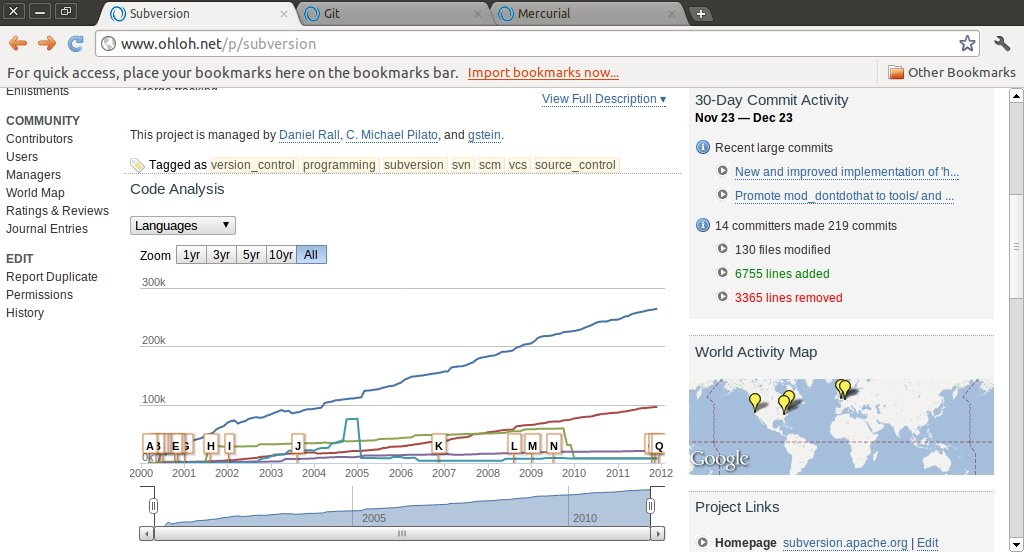
\includegraphics[width=15cm, keepaspectratio]{img/SVNohloh.jpg}
    \caption{\textit{Subversion Code Evolution}}
    \label{figure:svncodeevolution}
 \end{figure}

The next figure below shows the evolution of lines of code from Git Ohloh statistics page\footnote{http://www.ohloh.net/p/git}:

\begin{figure}[H]
    \centering
    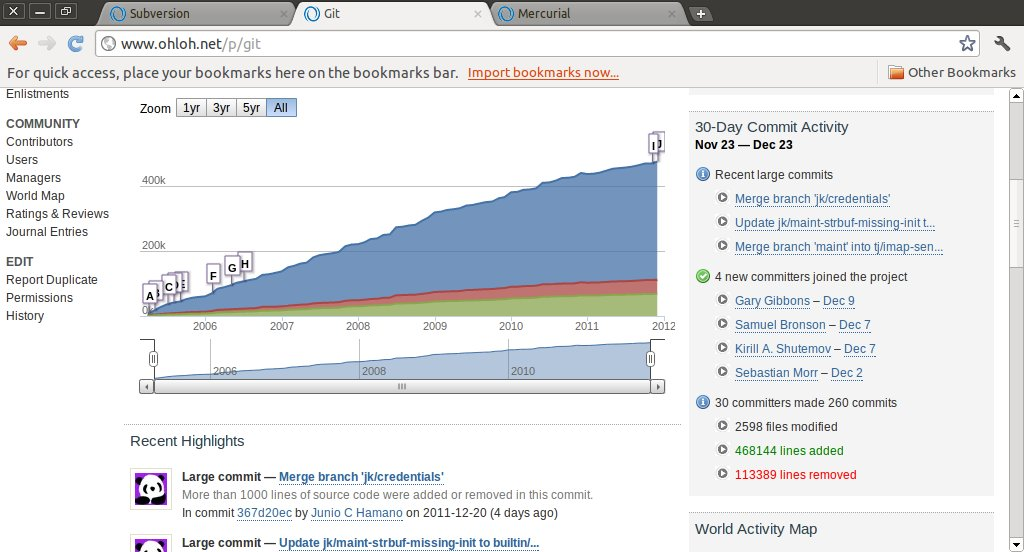
\includegraphics[width=15cm, keepaspectratio]{img/GITohloh.jpg}
    \caption{\textit{Git Code Evolution}}
    \label{figure:gitcodeevolution}
 \end{figure}

Finally, figure below shows the evolution of lines of code from Mercurial Ohloh statistics page\footnote{http://www.ohloh.net/p/mercurial}:

\begin{figure}[H]
    \centering
    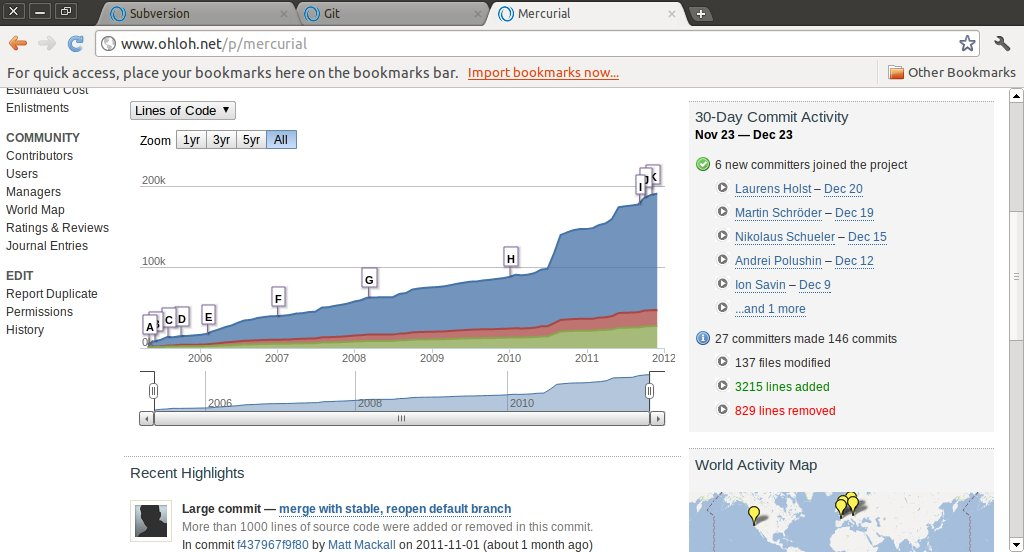
\includegraphics[width=15cm, keepaspectratio]{img/MERCURIALohloh.jpg}
    \caption{\textit{Mercurial Code Evolution}}
    \label{figure:mercurialcodeevolution}
 \end{figure}

If we compare the three figures we see that the evolution of lines of code commited to Subversion is not so high as the ones in Git and Mercurial, also an interesting parameter shown by Ohloh is that in the last month for Git project four new committers have joined the project, for Mercurial six new committers have joined the project and for Subversion no new committers have joined. This could mean that Git and Mercurial are younger projects but currently are in a more active status than Subversion which is a disadvantage for SVN.

According to the metric scores previously defined, Subversion is a long project (more than 10 years old) that also has an increasing number of lines of code production (not so explosive as in Git or Mercurial that is true ;-)) therefore the score for Subversion in this metric is 5.

\subsubsection{License}

Subversion is released under the Apache Public License (APL) v2.0\footnote{http://svn.apache.org/repos/asf/subversion/trunk/LICENSE}, all software produced by The Apache Software Foundation or any of its projects or subjects is licensed according to the terms of this license.

The Apache License is a “weak copy-left” license, being reciprocal in the same way that the GNU Lesser General Public License\footnote{http://www.gnu.org/licenses/lgpl.html} and the Mozilla Public License\footnote{http://www.mozilla.org/MPL/} are, the reciprocal clauses of the license force that changes and modifications to APL-licensed code need to be contributed back. Subversion trademarks and logo is out of the APL and belongs to the Apache Software Foundation. 

Currently the Free Software Foundation considers the Apache License compatible with the GNU Public License v3\footnote{http://www.gnu.org/licenses/gpl.html} but the Apache Software Foundation does not think the same\cite{APL}, therefore it is not clear if Subversion code could be mixed with GPL code.

The fact that the Subversion license is one of the
OSI-approved\footnote{http://www.opensource.org/licenses} FLOSS licenses is
clearly a strong point in favor of this solution, also being a weak copyleft
license allows to mix the product with proprietary code.

Therefore the final score for this metric is 5.

\subsubsection{Programming languages}

Figure below shows a pie diagram with the distribution of the different programming languages used in the implementation of Subversion:

\begin{figure}[H]
    \centering
    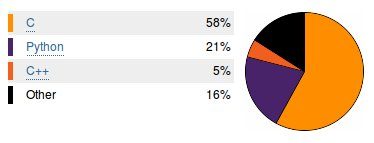
\includegraphics[width=10cm, keepaspectratio]{img/SVNlanguages.jpg}
    \caption{\textit{Subversion Programming Languages (Data retrieved from Ohloh)}}
    \label{figure:svnlanguages}
 \end{figure}

As we see in the figure, the core component of the SCM is written in C\footnote{http://subversion.apache.org/docs/api/1.6/modules.html} together with some C++ code (together they represent the 63\% of the code), the rest of the implementations are done using Python (21\%) or other languages (16\%).

The languages used to implement Subversion (C, C++, Python) are part of the most popular ones according to the latest surveys\footnote{http://www.tiobe.com/index.php/content/paperinfo/tpci/index.html}. Figure below shows Tiobe's survey on popularity of languages in December 2011:

\begin{figure}[H]
    \centering
    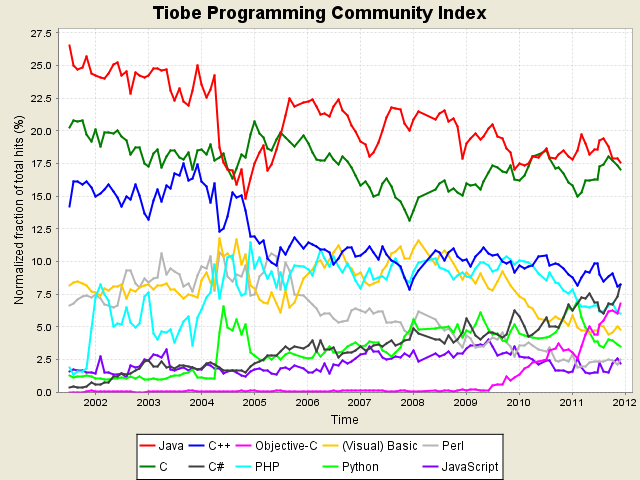
\includegraphics[width=12cm, keepaspectratio]{img/tiobe.png}
    \caption{\textit{Tiobe survey on most popular languages by Dec 2011}}
    \label{figure:tiobe}
 \end{figure}
 
The usage of popular languages for its implementation makes easier to find new developers to join the Subversion community, also as the core of the system is implemented using C/C++ which are very similar and stable languages that ensures a robust codebase for the tool.

\subsubsection{Contributors}

Regarding particular contributors, the project has a dedicated
page\cite{Contributors} where people can find all necessary info to start
working in the project as developer, translator etc... If I take a look at the
FLOSSMetrics data
provided\footnote{
http://docencia.etsit.urjc.es/moodle/mod/resource/view.php?id=6590} by Daniel
Izquierdo (our teacher in this subject) for the Subversion project I can analyze
that data using MySQL and R and get the total amount of commits within the
project which is 40869 commits. Also, I can get list of top-20 contributors of
the project:

\begin{figure}[H]
    \centering
    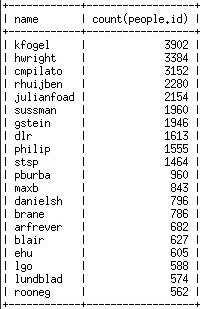
\includegraphics[width=5cm, keepaspectratio]{img/SVNcommitters.jpg}
    \caption{\textit{SVN Top-20 Commiters}}
    \label{figure:svncommitters}
 \end{figure}

From the above table and taking into account what I have already learnt about
the "Onion
Model"\footnote{
http://docencia.etsit.urjc.es/moodle/mod/resource/view.php?id=4177} in FLOSS
projects I can say that:

\begin{itemize}
\item  There is a group of three developers (kfogel, hwright and cmpilato) which
compose the "Core Team" of the project (by the way "kfogel" corresponds to Karl
Fogel, the author of one of the reference Open Source books "Producing Open
Source Software"\footnote{http://producingoss.com/}).
\item  Also there is a group of active "Co-developers" (from cmpilato to stsp)
that is composed of those developers that contribute frequently to the project
but do not have such an important role as the core.
\item The rest of the contributors (from the 11th until the latest one) are part
of the "Active Users" layer, these are people that contributes occasionally to
the project, mainly in specific parts of the code not so crucial.
\end{itemize}

With the total number of commits calculated before, I can easily calculate the
total amount of effort of the Core and Covedelopers layers together, this effort
is the 57\% so I can say that the effort in Subversion project is well-divided
between its members and if one of the key persons suddenly leaves the project
that would be a problem but it would not put in risk the project as there are
other people that can take the lead.

Figure below shows the density diagram of "Developers vs Number of commits", I
can see that it confirms what I have stated in terms of effort division within
Subversion, there is a big group of occasional commiters but also the small
group of key commiters is uniform.

\begin{figure}[H]
    \centering
    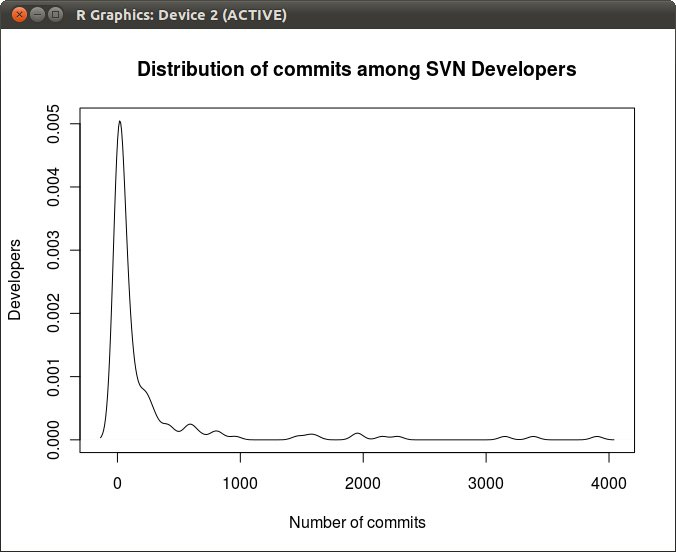
\includegraphics[width=10cm, keepaspectratio]{img/SVNdensity.jpg}
    \caption{\textit{SVN Developers vs Number of commits}}
    \label{figure:svndensity}
 \end{figure}

\subsubsection{Developers taking care of documentation}

Using the database dump from FLOSSmetrics for Subversion project, first we count the number of commits:
\begin{verbatim}
select count(*) from scmlog;
\end{verbatim}
giving a total of 40869 commits.
Now we count the commits mentioning the word ``documentation'':
\begin{verbatim}
select count(*) from scmlog where message like '%Documentation%' or message like '%documentation%';
\end{verbatim}
giving a total of 783 commits.
The relationship is 783/40869 = 0,019158, being between 1 and 5\% and so giving a score of 3 in the metric.

\subsubsection{Distance between the two most active authors}
Using the database dump from FLOSSmetrics for Subversion project, we count the commits of the two most active authors

\begin{verbatim}
select people.id, people.name, count(*) as numcommits from scmlog , people 
where people.id = scmlog.committer_id group by committer_id 
order by numcommits desc limit 2;

+-----+---------+------------+
| id  | name    | numcommits |
+-----+---------+------------+
|   2 | kfogel  |       3902 |
| 120 | hwright |       3384 |
+-----+---------+------------+
2 rows in set (0.26 sec)
\end{verbatim}

For normalizing the metric, we calculate the percentage of effort for each author: kfogel performs 3902 / (3902 + 3384) = 0,5355 (53,55\% of the two-people team effort). Hwright performs 3384 / (3902 + 3384) = 0,4644 (46,44\%). So the distance is 53,55 - 46,44 = 7,11\%, giving a score of 1.

\subsection{SWOT analysis}

Figure below shows the SWOT\cite{swot_analysis} diagram for Subversion: 

\begin{center}
\rowcolors{1}{}{}
    \begin{tabular}{ | p{1.5cm} | p{5cm} | p{5cm} |}
    \hline
    & Strengths & Weaknesses \\ \hline
    Internal Analysis & 
    Maturity/Stability (+10 years),
    Sustainability (ASF main supporter),
    Easy to use,
    Many GUI and IDE plugins,
    Good documentation (Books, Wiki, FAQ),
    Active Community (Mailing Lists)
    & Not centralized,
    No planned disrupting updates, 
    Slow roadmap\\ \hline
    & Opportunities & Threats \\ \hline
    External Analysis 
    & Supported by the ASF,
    Present in the main Spanish forges
    & May become obsolete, 
    Supported by less forges in the future\\ \hline
    \end{tabular}
\end{center}

The diagram summarizes the strong/weak points of Subversion that we have seen in
our previous analysis and also the opportunities/threats that come together with
this solution, this diagram is crucial for Amiguetes S.L. as it provides the
overall picture of Subversion and helps to decide if this SCM covers what is
expected or not:

\begin{itemize}
\item \textbf{Strengths}: The main strengths of Subversion are derived from the fact that it is really easy to use and provides lots of GUI and IDE plugins and also the project stability after more than 10 years of its creation, during this time the project has been able to create a very active community around it that ensures its future.
\item \textbf{Weaknesses}: Because the project it is in a stable status no major updates are planned and this is a disadvantage because we may need that a certain functionality which is important for us to be included as soon as possible in the next stable release but that next release is planned for a long time, also disruptive features that could be included in other less-mature SCMs as Git, Mercurial or Bazaar possibly will be included in SVN later than in the other tools. Another big challenge (possibly the biggest one) for SVN is that nowadays due to the distributed nature of many FLOSS projects it is desirable to use a distributed SCM and SVN is not like that and upgrading the tool to make it distributed is not a trivial change that I am not sure if the ASF is ready to implement at this stage of the project. 
\item \textbf{Opportunities}: The biggest opportunities for Subversion users comes with the support of the ASF, changes like the one we said before about doing SVN distributed can only be implemented by a huge community like the ASF, with their support the project could start boosting its development and bring brand new features that can compete with the rest of the SCMs. Apart from this, in the particular case of Amiguetes S.L., as we have seen the most important Spanish forges (Morfeo, Cenatic etc...) are supporting Subversion and this could be a change to move easily their code to one of this forges and start working with the forge in a straightforward way.
\item \textbf{Threats}: Because SVN is one of the oldest SCMs this could cause that it may become obsolete compared to the other solutions if its community is not able to implement on time new features that users are requesting, this thread will cause that less forges will include SVN support.
\end{itemize}

\newpage

%%%%%%%%%%%%%%%%%%%%%%%%%%%%%%%%%%%%%%%%%%%%%%%%%%%%%%%%%%%%%%%%%%%%%
\section{Appendix II: Git Analysis (Laura Arjona Reina)} \label{Git Appendix}

\subsection{Overview}
Git\cite{Git} is a cross-platform, distributed Open Source Software
Configuration Management (SCM) originally written by Linus Torvalds to be a
replacement for BitKeeper\footnote{http://www.bitkeeper.com/} SCM in the
\textbf{Linux kernel}\footnote{https://www.linux.com/} project. Git is focused
in speed and high performance.

The development started in the beginning of April 2005. The first ``official''
release was in December 2005, but it was used long before in production
environments (for
example, the Linux
Kernel development)\footnote{\url{http://marc.info/?l=git&m=113515203321888}}.
The last ``feature`` version is 1.7.8, released in December 2nd, 2011
\footnote{\url{http://article.gmane.org/gmane.linux.kernel/1223707}}.

The current leader is Junio C. Hamano (Linus Torvalds announced him as official
Git maintainer few months after the development
 started\footnote{\url{http://marc.info/?l=git&m=112243466603239}} and Hamano
lead the project since then). 

The software is mainly written in C and Perl languages.

Git is licensed under the terms of \textbf{GNU GPLv2}.

\subsubsection{Functionality}

Git is distributed version control system focused on speed and
high-performance. Among its main features we can list:
\begin{itemize}
 \item Distributed development. Each developer may have a local copy of the
entire development history, and commit changes while being disconnected.
 \item Support for different protocols: HTTP, FTP, rsync, git (plain and with
SSH).
\item Fast branching and merging, which allows strong support for non-linear
development.
\item Cryptographic authentication of history.
\item Toolkit design (collection of many small tools and scripts in the
low-level-end) and related tools and plugins (as Graphical User Interfaces,
Version Control Interface layers\dots) as frontends.
\end{itemize}

\subsubsection{Website, documentation (where is everything)}
You can find git source code in many different forges. Some of them are
Google Code (\url{http://code.google.com/p/git-core/}), GitHub
(\url{https://github.com/gitster/git}), Kernel.org
(\url{git.kernel.org/?p=git/git.git}) and all its mirrors of course,
SourceForge.net (\url{
http://git-core.git.sourceforge.net/git/gitweb.cgi?p=git-core/git-core}
), SourceForge Japan
(\url{http://git.sourceforge.jp/view?p=git-core/git.git}).

The main source of information for Git is the README file in any mirror of the
repository. In that file links to further sources of information can be found:
\begin{verbatim}
[..]
Please read the file INSTALL for installation instructions.
[...]
See Documentation/gittutorial.txt to get started
[...]
Many Git online resources are accessible from http://git-scm.com/
including full documentation and Git related tools.

The user discussion and development of Git take place on the Git
mailing list -- everyone is welcome to post bug reports, feature
requests, comments and patches to git@vger.kernel.org. To subscribe
to the list, send an email with just "subscribe git" in the body to
majordomo@vger.kernel.org. The mailing list archives are available at
http://marc.theaimsgroup.com/?l=git and other archival sites.

The messages titled "A note from the maintainer", "What's in
git.git (stable)" and "What's cooking in git.git (topics)" and
the discussion following them on the mailing list give a good
reference for project status, development direction and
remaining tasks.
\end{verbatim}

There is no official website of the project, as we can see, but we can consider
3 important websites to learn about the project:
\begin{itemize}
 \item  \url{http://git-scm.com/},
maintained by Scott Chacon, is a very good compilation of the most important
information and links. We can say that it is user-oriented.
 \item \url{https://git.wiki.kernel.org/} is the meeting point of the git and
Linux Kernel developers, and information about the community, integration with
other tools, events and news are found. We can say that it is
developer-oriented.
\item \url{http://git-blame.blogspot.com/} is the blog of Junio Hamano, Git
Maintainer. Most of the information posted there is about Git: announces of new
releases, project new challenges, open discussions...
\end{itemize}

\subsection{Sustainability}
\subsubsection{Developers and contributors (individuals, organizations,
companies)}
Git is a ``community-driven'' free software project in the sense that it is not
a product from any software company, however, some of the main developers are
paid developers for maintaining Git or git-related projects in important
companies (Junio Hamano and Shawn Pearce in
Google\footnote{http://www.ohloh.net/accounts/gitster and
http://www.ohloh.net/accounts/spearce}, Jeff King in
GitHub\footnote{https://github.com/blog/766-jeff-king-peff-is-a-githubber}).

\subsubsection{Users}
Many software projects use Git as software configuration management system.
Among them we can find\cite{Git}:
\begin{itemize}
 \item Git itself of course
 \item Linux Kernel
 \item Perl
 \item Eclipse
 \item Gnome
 \item KDE
 \item Qt
 \item Ruby on Rails
 \item Android
 \item PostgreSQL
 \item Debian
 \item X.org
\end{itemize}
On the other side, we can find that Git repositories are supported in many
used software forges (either for libre or privative software projects):
\begin{itemize}
 \item GitHub\cite{Github}: 1,216,063 people hosting over 3,586,678 git
repositories
 \item Google Code\cite{GoogleCode} supports Git since July, 2011.
 \item Gitorius
 \item BitBucket
 \item Assembla
 \item JavaForge
\end{itemize}

Among the important forges that do not support Git (yet), we have Launchpad and
CodePlex.

\subsection{Timeline, Roadmap, Future}
Since Git is a community driven project, there is not a clear long-term Roadmap
for the new features to include: the volunteer developers work on what they
want\footnote{There is an interesting discussion about this topic in the git
list (message \url{kerneltrap.org/mailarchive/git/2010/11/16/44916} and
follow-ups)}.

However, one of the main worries of the Git developers are to facilitate the
work of the Linux Kernel development, and subsequently, enhance the main
features of this SCM: speed and high performance specially for big projects.

From Git Maintainer's blog \url{http://git-blame.blogspot.com/} we can learn
that important features to include in next release (1.7.9)
are\footnote{\url{
http://git-blame.blogspot.com/2011/12/moving-forward-to-179.html}}:
\begin{itemize} 
 \item Better and more auditable communication in pull based workflow by
supporting electronically signed pull requests that records more meaningful
branch description;
 \item More pleasant end-user experience by providing credential helper API to
allow platform native keychain implementations to supply authentication material
during "git push" and "git pull";
 \item i18n of messages out of the end-user facing programs;
 \item Better large-contents support.
\end{itemize}

Junio Hamano also announces in his blog the different releases, and when one
release is announced, the development cycle time estimation for the next
release is announced too.

\subsection{OpenBRR details and references}

Taking as a starting point the OpenBRR Git template that my class group
implemented in the "Project Evaluation" subject, the spreadsheet has been
changed or improved in several ways:
\begin{itemize}
 \item All weights in Category Ranking and Category Rating and Metrics
sheets have been changed to match Amiguetes S.L. requirements (more details in
section \ref{OpenBRR_application}).
 \item Functionality sheet has been rewritten with functionality
aspects that match Amiguetes S.L. requirements.
 \item The ``Quality'' category was not fulfilled in the original template.
This category is measured with two metrics related to software releases and
four more metrics related to bug tracking. The metrics about software releases
have been fulfilled, but the ones about bug reporting and tracking are
difficult to measure in Git project, since the community does not use a bug nor
issue tracking system, but only the official mailing list. Even the bugs are
not numbered and the subject of the mail messages related to a reported bug
change frequently (and the recommended tag [BUG] is rarely used). This does not
mean that the developer community does not care about bugs in Git project, but
the handling of the reported issues is not standardized, which is in fact a
limitation for improving the quality of the project. For this reason,
bug-related metrics have been marked with the lowest score.
\item Other categories' metrics have been fulfilled or corrected
(Performance tuning, Professional support, 3rd party plugins, difficulty to
enter the core developer team) and references for metric sources added to other
metrics.
\item New metrics have been included and scored according to the descriptions
in section \ref{OpenBRRimprovements}.
\end{itemize}

The final version of the template is available in our collaborative repository
under:

\url{
https://gitorious.org/mswl-eval/mswl-eval/blobs/master/ProjectEvaluation_Report/
OpenBRR_Templates/BRR_Template_Git_larjona.ods}

The final score for Git is 3,59, that means is good solution for
Amiguetes S.L. 

From the template results we can derive the following conclusions:

\begin{itemize}
\item \textbf{Functionality Rating}: This is a key issue in our analysis, and
Git obtains an extraordinary good result, because ``git-core'' can be
configured to make many different things and the design is very modular
and efficient, with many tools or commands that extend the functionality.
\item \textbf{Usability}: For Amiguetes S.L. it is essential that the selected
SCM is easy to use as not everyone in the team is familiarized with version
control tools. Git is basically a set of command-line tools, easy to install
and use, once you learn the basics. For people needing graphical clients, many
tools are available so each person may decide the one that suites best to her
skills.
\item \textbf{Quality}: This seems a weak point of Git. The software has proven
its quality (by being used in many production systems with strong requirements,
as the Linux Kernel Development), but that quality is threatened by the fact
that the development depends on a very small set of committers (and highly on
the Git maintainer), and the handling of bugs, support requests, roadmap etc is
performed in a very home-made way, without tools that standardize the workflows
and allow the scalability of the development community. However, quality is a
low-weight category for the requirements of Amiguetes S.L. so the low score of
Git in this aspect does not affect too much to the global score.
 
\item \textbf{Security}: In terms of Security applies the same as above. There
are not recent public security holes discovered in Git; this may mean that it
is a secure tool, but also that security holes are not handled in a standardized
way. But no advanced security is required for Amiguetes S.L. so Git passes well
this ``test''.

\item \textbf{Performance}: Git obtains a good score in performance, indeed
this is one of the main goals of this SCM.
\item \textbf{Scalability}: In principle Amiguetes S.L. is going to be a small
company and it is not intended in the future a huge grow, therefore scalability
is not a key feature although it is well covered in Git, specially because of
its distributed nature.

\item \textbf{Architecture}: Git's modularity and popularity have made possible
to find many plugins and tools to integrate Git with development IDEs, forges,
continuous integration systems... This category is low-weighted in the
Amiguetes OpenBRR sheet since main functionality is measured in the
``Functionality'' category/sheet, but Git still obtains the highest possible
score in the Architecture category.

\item \textbf{Support}: For a small company like our example use case the
support is an important factor. Git obtains the best possible score in this
category, for two main reasons: following the very active Git mailing list,
where you don't need to be subscribed to send emails and even patches, you
obtain
the most important feedback from the community. On the other side, Git's
popularity and the increasing adoption have created a business niche for many
companies offering git hosting along with git training and support, so although
the Git Developer teams does not provide professional support, many of their
members work as paid git developers in some companies or give training or talks
about git in a professional way, but also making publicly available all the
documentation (talk slides, videos, even books published with Creative Commons
licenses), so the support is available for small git users too, not only for
the companies able to pay for it.
 
\item \textbf{Documentation}: As we saw in the previous sections there are
different publications and web sites available with Git-related
documentation. Everybody is allowed to participate in the Git mailing list and
the git developers, a small team, discuss and decide which changes to include
in the ``master'' branch, so they act as quality filters to the information and
features developed. We also find that the git maintainer and git developers also
care about documentation, not only the source code.

\item \textbf{Adoption}: Here we see that Git has been adopted as the reference
SCM solution for several stable FLOSS projects and public forges. In addition
to this, books about Git have been published, and GitHub, the biggest software
forge with git support, has been a key factor to improve the adoption of this
tool in the software environments.

\item \textbf{Community}: Git is supported by an very active, small community of
developers plus a long-tail group of many contributors, in a typical ``onion
model'' software project. This makes the project advance, and the only weak
point is the fact that the git maintainer, Junio Hamano, is performing most of
the work in the development team, what puts the project in danger if he gets
out for some time, for any reason. But fortunately, it seems he is happy with
the ongoing of the project and his plans are continuing working in Git (indeed
he has ben hired by Google to ensure this).
 
\item \textbf{Professionalism}: The project is driven by individuals, the git
developers and the git maintainer, what is not well considered in this
category. However, the team works well and reviews all the submitted work from
external contributors, which ensures professionalism despite of being a certain
company behind Git or not.
\end{itemize}

\subsection{Additional metrics and evaluations}


\subsubsection{Longevity}
As mentioned before, Git development began in April 2005, and it was quickly
put in production sites. 

Figure \ref{figure:gitcodeevolution2} shows the evolution of lines of code
from Git Ohloh statistics page\footnote{http://www.ohloh.net/p/git}:

\begin{figure}[H]
    \centering
    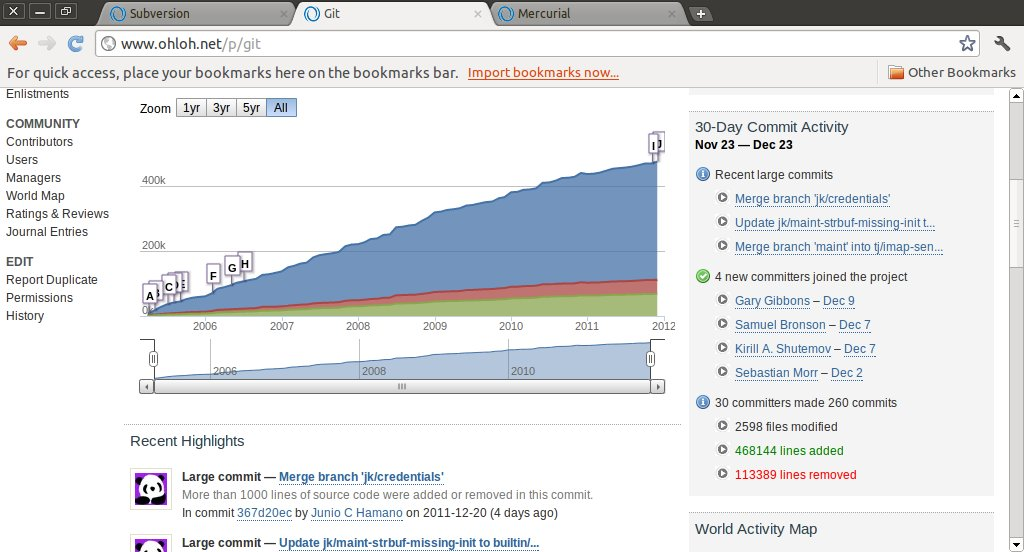
\includegraphics[width=15cm, keepaspectratio]{img/GITohloh.jpg}
    \caption{\textit{Git Code Evolution}}
    \label{figure:gitcodeevolution2}
 \end{figure}

An interesting parameter shown by Ohloh is that in the last month for Git
project four new contributors have joined the project\footnote{Ohloh mentions
the word ``committer'' for them, but if we look at their ``commits'', we find
that their commits have been signed off by other committers (mostly the Git
maintainer Junio Hamano)}.

According to the metric scores previously defined, Git is a medium-aged project
(between 5 and 10 years old) that also has an increasing number of lines of code
production therefore the score for Git in this metric is 3.

\subsubsection{License}

The fact that the Git license (GPLv2) is one of the
OSI-approved\footnote{http://www.opensource.org/licenses} FLOSS licenses is
a strong point in favor of this solution, although being a strong copyleft
license it does not allow to mix the product with proprietary code.

Therefore the final score for this metric is 3.

\subsubsection{Programming languages}

Figure \ref{figure:gitlanguages} shows a pie diagram with the distribution of
the different programming languages used in the implementation of Git:

\begin{figure}[H]
    \centering
    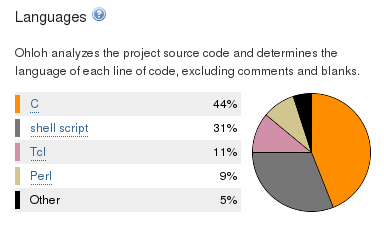
\includegraphics[width=10cm, keepaspectratio]{img/Gitlanguages.png}
    \caption{\textit{Git Programming Languages (Data retrieved from
Ohloh)}}
    \label{figure:gitlanguages}
 \end{figure}

As we see in the figure, the core component of the SCM is written in
C together with shell scripts.

C is one of the most popular languages according to the latest
surveys\footnote{
http://www.tiobe.com/index.php/content/paperinfo/tpci/index.html}. Figure
\ref{figure:tiobe}
showed Tiobe's survey on popularity of languages in December 2011, and we can
conclude that the usage of the C popular language for its implementation makes
easier to find new developers to join the Git community, but we also need to
consider that some parts are written in Tcl which is not a popular language
nowadays, and also we cannot determine anything about the ``shell scripts'',
since they are popular among sysadmins but not much used by developers.

\subsubsection{Contributors}
Git is an excelent example of a project that matchs the Onion
Model\cite{Onion}, with its leader performing a huge part of the work (we will
see it later), a small set of people with commit permissions and co-developing
the tool\footnote{In FLOSSMetrics database: select count(id) from people
where id in (select distinct committer\_id from scmlog); gives 30}, and a very
big group of contributors submitting patches (the rest of
``authors'')\footnote{In FLOSSMetrics database: select count(id) from
people; gives 957.}.

We can query the FLOSSMetrics data in order to obtain the top-20 contributors
and their commits in the history of the project:
\begin{verbatim}
 select people.name, scmlog.author_id, count(*) as numcommits
from people, scmlog where people.id = scmlog.author_id 
group by people.id order by numcommits desc limit 20;
+-------------------------+-----------+------------+
| name                    | author_id | numcommits |
+-------------------------+-----------+------------+
| Junio C Hamano          |         5 |      10502 |
| Shawn O. Pearce         |       224 |       1327 |
| Linus Torvalds          |         1 |       1101 |
| Johannes Schindelin     |        54 |        729 |
| Jeff King               |       179 |        695 |
| Jonathan Nieder         |       530 |        557 |
| Jakub Narebski          |       189 |        488 |
| Eric Wong               |       118 |        466 |
| *var Arnfj*r* Bjarmason |       798 |        419 |
| Nicolas Pitre           |        16 |        349 |
| Johannes Sixt           |       227 |        328 |
| Paul Mackerras          |        13 |        323 |
| Rene Scharfe            |        17 |        289 |
| Christian Couder        |       184 |        283 |
| Simon Hausmann          |       298 |        252 |
| Nguyen Thai Ngoc Duy    |       300 |        252 |
| Brandon Casey           |       274 |        244 |
| Petr Baudis             |         4 |        221 |
| Thomas Rast             |       529 |        210 |
| Alex Riesen             |        96 |        210 |
+-------------------------+-----------+------------+
20 rows in set (0.27 sec)
\end{verbatim}

If we sum the commits of Junio Hamano and Shawn Pearce, we find that they
perform more than 40\% of total commits. We believe that this distribution of
effort is a little bit risky for the sustainability of the community (it would
be positive for other aspects, however). So for this metric of Community git
has a low score: 1. 

\subsubsection{Developers taking care of documentation}
Using the database dump from FLOSSmetrics for Git project, first we count
the number of commits:
\begin{verbatim}
select count(*) from scmlog;
\end{verbatim}
giving a total of 28029 commits.
Now we count the commits mentioning the word ``documentation'':
\begin{verbatim}
select count(*) from scmlog where log like '%Documentation%' 
                            or log like '%documentation%';
\end{verbatim}
giving a total of 2371 commits.
The relationship is 2371/28029 = 0,08459, being more than 5\% and so
giving a score of 5 in the metric.

\subsubsection{Distance between the two most active authors}
Using the database dump from FLOSSmetrics for Git project, we count the commits
of the two most active authors
\begin{verbatim}
select people.id, people.name, count(*) as numcommits from scmlog , people 
where people.id = scmlog.author_id 
group by author_id order by numcommits desc limit 2;

+-----+-----------------+------------+
| id  | name            | numcommits |
+-----+-----------------+------------+
|   5 | Junio C Hamano  |      10502 |
| 224 | Shawn O. Pearce |       1327 |
+-----+-----------------+------------+
2 rows in set (0.18 sec)
\end{verbatim}
For normalizing the metric, we calculate the percentage of effort for each
author: Junio C. Hamano performs 10502 / (10502 + 1327) = 0,8878 (88,78\% of the
two-people team effort). Shawn O. Pearce performs 1327 / (10502 + 1327) = 0,1121
(11,21\%). So the distance is 88,78 - 11,21 = 77,57\%, giving a score of 1.

\subsection{SWOT analysis}
Table below shows the SWOT\cite{swot_analysis} diagram for Git:
\begin{center}
    \begin{tabular}{ | p{1.5cm} | p{5cm} | p{5cm} |}
    \hline
	  & \textbf{Strengths} & \textbf{Weaknesses} \\ \hline
    \textbf{Internal Analysis} & 
    Easy to use,
    Many GUI and IDE plugins,
    Good documentation (Books, Wiki, FAQ),
    Active Community ,
    Distributed,
    Strong copyleft license guarantees new versions be FLOSS
    & High dependence on Git Maintainer,
    Uncertain roadmap, 
    No professional handling of bugs and vulnerabilities \\ \hline
    & \textbf{Opportunities} & \textbf{Threats} \\ \hline
    \textbf{External Analysis} & 
    Great level of adoption,
    Present in the main forges and modern ones,
    Existence of external support and services
    & Not guaranteed economic sustainability,
    Companies may get much influence in the project by hiring the Git maintainer
    Goodness of the ``core'' product does not mean goodness of the 3rd party
tools and wrappers    
\\ \hline
    \end{tabular}
\end{center}

Most of the different aspects of this SWOT table have already been explained in
former sections. The table may help Amiguetes S.L., in the case of deciding
to deploy Git for their infrastructure, to pay attention to certain aspects
that may announce future dangers of the Git project, and so, they would take
advance in moving to a different SCM and not fail with Git, in this is the case.

\newpage

%%%%%%%%%%%%%%%%%%%%%%%%%%%%%%%%%%%%%%%%%%%%%%%%%%%%%%%%%%%%%%%%%%%%%
\section{Appendix III: Mercurial Analysis (Cesar Valiente Gordo)}
\label{Mercurial Appendix}

\subsection{Overview} \label{Overview}

\textbf{Mercurial}\footnote{http://mercurial.selenic.com/} is a distributed
version control system.
This SCM was started with the intention to be a replacement for
BitKeeper\footnote{http://www.bitkeeper.com/} in the
\textbf{Linux}\footnote{https://www.linux.com/} project in April 19, 2005 by
Matt Mackall.

Mercurial is mainly implemented in \textbf{Perl}, and \textbf{Python}. It's
supported on Windows and Unix-like systems as Linux, FreeBSD, MacOS X, etc.
Mercurial is basically a command line program but there are some
GUIs\footnote{Graphic User Interface} 

Mercurial is licensed under the terms of \textbf{GNU
GPLv2}\footnote{http://www.gnu.org/licenses/gpl-2.0.html}.

\subsubsection{Functionality} \label{Functionality}

Mercurial was designed to provide high performance and scalability is
decentralized, allows fully distributed collaborative development, is robust
handling managing both plain text and binary files, and has advanced branching
and merging capabilities, while remaining conceptually simple.

As a important things which Mercurial has into an account are it has an
integrated web interface and has also taken steps to ease the transition for
\textbf{SVN} users.

Mercurial uses \textbf{SHA-1} hashes to identify revisions. For repository
access via network, Mercurial uses \textit{HTTP-based protocol} that seeks to
reduce round-trip (RTT) requests, new connections and data transferred.
Mercurial also work over \textbf{ssh} where the protocol is very similar to the
HTTP-based protocol.
By default, it uses a \textit{3-way merge}\cite{3-way merge} before calling
external merge tools.

\subsubsection{Website, documentation (where is everything)} \label{Website,
documentation (where is everything)}

The Mercurial website where any user can find all information regarding the
packages to install, different versions, etc. is
\url{http://mercurial.selenic.com/}.
This website besides the mentioned information also includes the next sites:
\begin{itemize}
 \item Download the binaries\footnote{http://mercurial.selenic.com/downloads/}.
 \item Download the source code\footnote{http://selenic.com/hg}.
 \item A guide\footnote{http://mercurial.selenic.com/guide/}.
 \item Extensions to use with
Mercurial\footnote{http://mercurial.selenic.com/wiki/UsingExtensions}.
 \item News and wiki\footnote{http://mercurial.selenic.com/wiki/}.
 \item Information about the Mercurial
sponsors\footnote{http://mercurial.selenic.com/sponsors/}.
\end{itemize}


\subsection{Sustainability} \label{Sustainability}

As we've said before, in the Mercurial website we can find the major
sponsors\footnote{http://mercurial.selenic.com/sponsors/} which give Mercurial
the assurance to be sustainable for long time.
The most important of them are the \textit{Gold Sponsors} which investment
\$20000 and above, they are:
\begin{itemize}
 \item \textit{Google}\footnote{http://www.google.com/}.
 \item \textit{Fog Creek Software}\footnote{http://www.fogcreek.com/}.
 \item
\textit{Microsoft}\footnote{http://www.microsoft.com/en-us/default.aspx}.
\end{itemize}

After them we can find the \textit{Silver Sponsors} with an investment between
\$5000 to \$19999, they are:
\begin{itemize}
 \item \textit{Atlassian}\footnote{http://www.atlassian.com/}.
 \item \textit{Jane Street Capital}\footnote{http://www.janestcapital.com/}.
 \item \textit{Allston Trading LLC}\footnote{http://www.allstontrading.com/}.
\end{itemize}

And finally, we have the \textit{Bronze Sponsors} with an investment between
\$1000 to \$4999 like:
\begin{itemize}
 \item \textit{Mozilla Foundation}\footnote{http://mozilla.org/}.
 \item \textit{Symbian Foundation}\footnote{http://symbian.org/}.
 \item \textit{Python Software Foundation}\footnote{http://python.org/psf}.
 \item \textit{Jet Brains}\footnote{http://www.jetbrains.com/}.
\end{itemize}

\subsection{Users} \label{Users_mercurial}

Mercurial is used as the SCM for a lot of important software projects, also is
included in very important privative forges and FLOSS.

An example of projects which use Mercurial are:
\begin{itemize}
 \item Adium. 
 \item Illumos.
 \item Mercurial.
 \item Mozilla.
 \item Netbeans.
 \item OpenJDK.
 \item OpenIndiana.
 \item OpenOffice.org.
 \item Python.
 \item Symbian OS.
 \item Nokia Maps.
 \item Tuenti.
 \item Vim.
 \item W3C. 
\end{itemize}

And forges which use Mercurial:
\begin{itemize}
 \item CodePlex\footnote{http://www.codeplex.com/}.
 \item Google Code\footnote{http://code.google.com/}.
 \item SourceForge\footnote{http://sourceforge.net/}.
 \item GNU Savannah\footnote{http://savannah.gnu.org/}.
 \item BerliOS\footnote{http://www.berlios.de/}.
\end{itemize}

As we can see very important projects and very important forges use Mercurial,
so this is very good for the health of Mercurial project.

\subsection{Timeline - Roadmap - Future}

In the Mercurial website regarding the \textit{project
roadmap}\footnote{http://mercurial.selenic.com/wiki/RoadMap} we can see how
since December 31, 2007 in the version 1.0 we don't have new features for new
ones, but we can see the planned new features (unknown dates):
\begin{itemize}
 \item Partial Clone\footnote{http://mercurial.selenic.com/wiki/PartialClone}.
 \item Nested
Repositories\footnote{http://mercurial.selenic.com/wiki/NestedRepositories}
 \item inotify on Windows/OS X.
 \item Improved merging workflow.
 \item Fix case collision bugs.
 \item Some translations in place.
 \item Experimental support for history punching (TrimmingHistory)
 \item Faster incoming (rsync-like algorithm) 
\end{itemize}

We think this road map is not updated, since the last \textit{new features}
info in 2007, and after that this information, we can not being too confident
about it.

\subsection{OpenBRR details and references}

As previously we did in the appendices \ref{SVN Appendix} and \ref{Git Appendix}
taking as a baseline the OpenBRR Mercurial template implemented in the ”Project
Evaluation” class and completing the sheets that we didn't have finished, I have
updated the features rating according to the requisites of our Amiguetes S.L.
use case, the final version of the template is available in our collaborative
repository under:
\url{https://gitorious.org/mswl-eval/mswl-eval/blobs/master/ProjectEvaluation_
Report/OpenBRR_Templates/BRR_Template_Mercurial_cvaliente.ods}

We can see now a brief summary about the twelve different methodologies used
and how they fit in Mercurial.

\begin{itemize}
\item \textbf{Functionality Rating:}
This is the most important feature in our SCM study, Mercurial covers the most
important 
things we need to cover Amiguetes S.L. requisites, but also provides a new and 
important feature if we compare this SCM with others like SVN or CVS, and is the
distributed functionality of this SCM.
Distributed SCM like Mercurial or Git are maybe more versatile because the allow
developers of different location work with is own copy of the repository (a
complete copy), 
in his own computer to later merge the changes to the global branch, having the
complete
copy also means that the developer has all data, like different versions, can
create
studies based in all changes, etc.

\item \textbf{Usability:}
This is also a very important point in the deploy and use of this SCM in
Amiguetes S.L.
the people who are going to use this SCM are used to use CVS and not distributed
SCM, but they are willing
to learn about these kind of \textit{news} distributed SCM, Mercurial is not
difficult to use
but as all transitions to new technologies is very important if the people want
to learn and use it quickly.

\item \textbf{Quality:}
Amiguetes S.L. tries to be a software company a startup, and tries to be a
flexible company which
they don't want to spend a lot of time in quality process regarding their SCM,
they prefer a SCM which
will be flexible, stable and easy to use, in fact another one to fit to several
standards but in the other
side will be really difficult to use, anyway, Mercurial fits perfectly with a
good level of quality and a prove of that
is the amount of clients and users who use this SCM along the world.

\item \textbf{Security:}
Like the previous point, Amiguetes S.L. needs a SCM which offers a good point of
security, but is not really mandatory
that Mercurial will be the most secure SCM, anyway, with plugins Mercurial
offers extra functionality which
covers this part.

\item \textbf{Performance:}
Mercurial offers a good ratio of performance and being distributed the charge in
the network also will be decreased.

\item \textbf{Scalability:}
As a distributed SCM the scalability is a fact in Mercurial, as a distributed
system, the scalability is completely
possible and in fact is the reason to be in Mercurial.

\item \textbf{Architecture:}
Mercurial is building to be a complete SCM by itself but also provides a set of
plugins which give more functionality, and sturdiness to this SCM, plugins like
the ones which offer PGP, or integration with MyLyn, or another tools are
very important for any FLOSS community or company.

\item \textbf{Support}:
Mercurial has a really big community behind it so is easy to find the fix for
near any problem you have with this SCM, also and we think ant the beginning for
Amiguetes S.L. is not necessary, it's possible to find companies which offer
professional support for
Mercurial\footnote{http://www.clearvision-cm.com/mercurial.html}.

\item \textbf{Documentation:}
This feature is really close to the previous one and as a well known FLOSS
project is possible to find a lot of documentation \textit{"official"} in its
own website and created by third parties (developers or companies).

\item \textbf{Adoption:}
As we can see in the \textbf{section \ref{Users_mercurial} (Users)} Mercurial is
used by a lot of customers (developers and companies) along the world, between
this companies we can find since developer communities, SME's or big
enterprises.
Little by little this kind of SCM (like Git) are growing a lot in comparison
with the older CVS or SVN SCMs.

\item \textbf{Community:}
As a well known FLOSS project used by thousand of people around the world,
Mercurial has a very important and big community around it, not only the mainly
developers, but others who use Mercurial in their projects, write in forums,
write documentation, ask questions, etc.
As a bad point Mercurial is not under the manage of any FLOSS foundation, it's
managed by its main developer and the others who develop Mercurial with him, so
is much better if the project would have a foundation as SVN with Apache
Software Foundation, to preserve the rights, code, brands, etc.

\item \textbf{Professionalism:}
The way to work in Mercurial is not the way as work in bigger and well organized
FLOSS communities like Apache Software Foundation, so as the previous point,
would be much better if the project would be managed by a similar foundation,
but anyway, the way to work in Mercurial is as we can see in the data about
developers is similar to any other FLOSS projects, with contributors, main
developers, users, etc. following the Onion Skin way.
\end{itemize}

\subsection{Additional metrics and evaluations}

To know data about the way how is building Mercurial and data regarding the
code, we can use the website \textbf{Ohloh}\footnote{http://www.ohloh.net/} and
\textbf{FLOSSMetrics}\footnote{http://flossmetrics.org/} where we can check and
study the following aspects:

\subsubsection{Longevity} \label{longevity_mercurial}

As we've seen in the \textbf{Appendix \ref{SVN Appendix}} the oldest SCM we've
studied is SVN, which is a really good thing, but as we've said in that
section, the distributed SCM as Mercurial and Git are much more actives, this
is really good, but as we've said for a company usually is much better having a
really stable and robust product.

The figure below shows the evolution of lines of code from Mercurial Ohloh
statistics page\footnote{http://www.ohloh.net/p/mercurial}:

\begin{figure}[H]
    \centering
    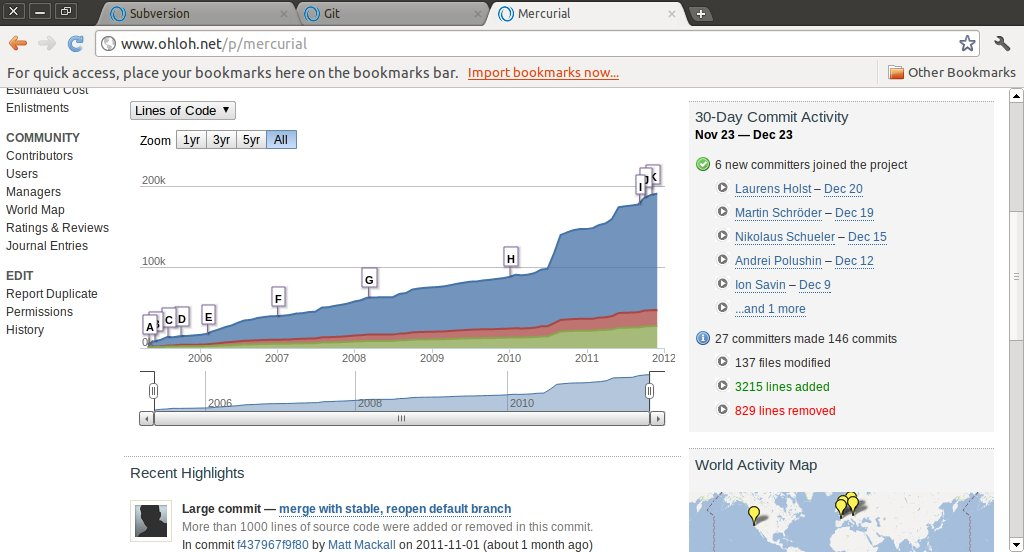
\includegraphics[width=15cm, keepaspectratio]{img/MERCURIALohloh.jpg}
    \caption{\textit{Mercurial Code Evolution}}
    \label{figure:mercurialcodeevolution2}
 \end{figure}

As we've seen in the three appendix (SVN) is being developed now much slower
than the other two (Git and Mercurial which both are younger projects), but it
doesn't mean that the project is being to be abandoned, as we know, SVN is being
developed since long time ago, and it's really stable, the other two, are
stables also but are growing.

According with the rating we talked before, Mercurial is a project with new and
lot of changes with an very high grow but is not as old as SVN so the score for
Mercurial in this metric is 3.

\subsubsection{License} \label{license_mercurial}

As we've said in the Mercurial introduction, this SCM is licensed under the
terms of \textbf{GNU GPLv2} so is a reciprocal (strong) FLOSS license, that it
means is not possible to release derivative products under another license
neither release it under any privative license (is a copyleft license).

This license is approved for the three most important FLOSS
communities/organizations,
\textbf{FSF}\footnote{http://www.gnu.org/copyleft/gpl.html},
\textbf{OSI}\footnote{http://www.opensource.org/licenses/alphabetical} and
\textbf{Debian Free Source Guidelines
(DFSG)}\footnote{http://wiki.debian.org/DFSGLicenses}.

As this project (Mercurial) we pretend to use in the company Amiguetes S.L.
and for enterprises we think the permissive licenses give more liberty to the
users, and because this license is FSF, OSI, and DFSG compatible we give a
final score of 3 for this metric.



\subsubsection{Programming languages} \label{Programming languages}

As we can see in the \textit{Figure \ref{figure:mercurial_languages}},
Mercurial is developed using basically Perl and Python with more of 90\% in
total.

The rest is for C and shell script languages (and in a minor way Vim script).

\begin{figure}[H]
    \centering
    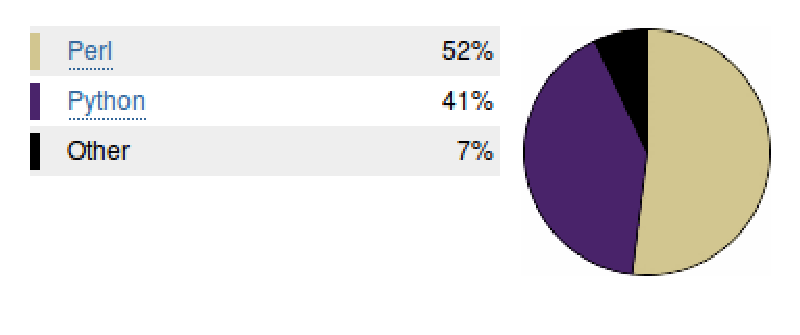
\includegraphics[width=10cm, keepaspectratio]{img/mercurial_languages.pdf}
    \caption{\textit{Programming languages used in Mercurial}}
    \label{figure:mercurial_languages}
 \end{figure}

As an interesting thing about the programming languages used in this project,
we can think about how it easy would be to be involved in this project if for
instance a developer would wish, here the language programming used is really
important since if the project uses languages with not a really hard barrier to
learn if you don't know about it the collaboration will be easy, in the other
side, if the project use a language which is difficult to understand and you
don't know about it, you, surely, will think a lot about to be involved in this
project or going to another different.

As we see, Mercurial is developed in Python at most and in Perl, both really
famous and easy going languages programming, besides, in the \textit{FLOSS
world}
these both languages are really used in a lot of different projects, so is
really easy that a developer who want to be involved already know about it.

In the other side we need to have into account the number of different
programming languages, I think, personally, that a FLOSS project which uses
more than one language programming is very important and enriches the project,
because give the opportunity to other developers who maybe don't know about one
of the languages used but any other used yes to be involved in a project who
thinks is really interesting.

As a curious thing in the Wikipedia report regarding Mercurial\cite{Mercurial
(Wikipedia)}, 
we can see how it's written \textit{"It is mainly implemented using the Python
programming language, but includes a binary diff implementation written in C"}
this affirmation was true, but not since \textbf{September 2010} when Perl
language programming exceeded to Python as the most important programming
language used in Mercurial.
As we can see in the \textbf{Figure \ref{figure:mercurial_languages_evo}} now
in \textbf{January 2012}, the most important language is Perl following of
Python, being C which Wikipedia says is the 2nd most important language the 3rd
one.

So finally, and following the mentioned valuation way to value this metric,
Mercurial has a score of 3.


\begin{figure}[H]
    \centering
    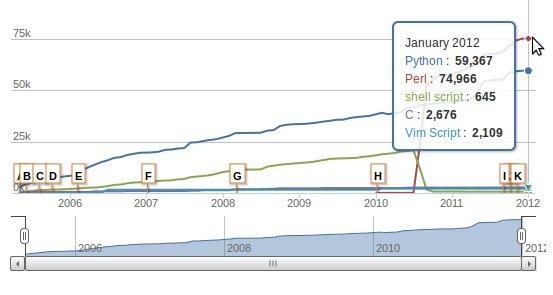
\includegraphics[width=10cm, keepaspectratio]{img/mercurial_languages_evo.jpg}
    \caption{\textit{Programming languages evolution used in Mercurial}}
    \label{figure:mercurial_languages_evo}
 \end{figure}

\subsubsection{Contributors} \label{Contributors}

Along the entire life of this project it has a lot of developers, but as most of
FLOSS project we have a set of main developers who perform the most number of
commits, this stats are regarding since the 1st day of the project until
December 8th, 2011 (this month).

The total amount of commits in Mercurial is \textbf{15590}, and the most
important developers are:

\begin{itemize}
 \item Matt Hackball: 3571 commits, 22\%.
 \item Martin Geisler: 1351 commits, 8\%.
 \item Thomas Arendsen Hein: 1004 commits, 6\%.
 \item Patrick Mezard: 972 commits, 6\%.
 \item Benoit Boissinot: 933 commits, 5\%.
 \item Adrian Buehlmann: 322 commits, 2\%.
 \item Christian Ebert: 242 commits, 1\%.
 \item Idan Kamara: 141 commits, 0\%.
 \item Others: 7054 commits, 45\%
\end{itemize}

To help us to see much better this we can check the \textbf{Figure
\ref{figure:mercurial_commits}}:

\begin{figure}[H]
    \centering
    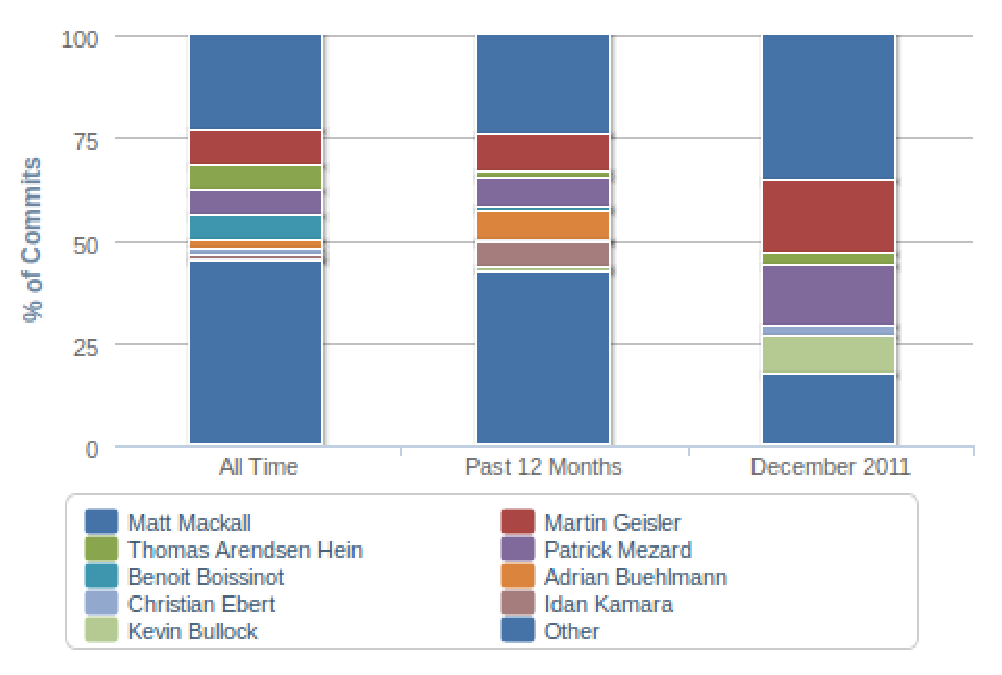
\includegraphics[width=12cm, keepaspectratio]{img/mercurial_commits.pdf}
    \caption{\textit{Commits in Mercurial}}
    \label{figure:mercurial_commits}
 \end{figure}

As we can see the most important developer is \textbf{Matt Hackball}, Mercurial
creator, is close to the quarter of the total of commits, after him is
\textit{Martin Geisler} but really far from his commits, and if we following
seeing the list we can appreciate how the \textbf{onion skin} model in FLOSS
projects also is really appreciate here in this project, with a very strong and
important group of developers (here maybe the top 5) and the rest, but one thing
is true, almost the half of the commits are from others developers who maybe
commit a few times, so this project although has a top group of developers,
without the rest of them, this project won't be possible.

As a not, we can see how the sum of the percentage is not 100\%, is a 95\%, so
the rest of the 5\% unknown commits could be from different developers who
they are unknown (also is different the commit author than the authorship).

Following the mentioned before about the valuation of this metric, Mercurial
has a score of 3 (four developers have developed at least 40\% of the code).

\subsubsection{Developers taking care of documentation}
Using the database dump from FLOSSmetrics for Mercurial project, first we count
the number of commits:
\begin{verbatim}
select count(*) from scmlog;
\end{verbatim}
giving a total of 15555 commits.
Now we count the commits mentioning the word ``documentation'':
\begin{verbatim}
select count(*) from scmlog where log like '%Documentation%' or log like
'%documentation%';
\end{verbatim}
giving a total of 78 commits.

The relationship is 78/15555 = 0,00501, being less than 1\% and so giving a
score of 1 in the metric.


\subsubsection{Distance between the two most active authors}
Using the database dump from FLOSSmetrics for Mercurial project, we count the
commits of the two most active authors

\begin{verbatim}
select author, count(*) as numcommits from scmlog 
group by author order by numcommits desc limit 2;

+---------------------------------------------+------------+
| author                                      | numcommits |
+---------------------------------------------+------------+
| Matt Mackall <mpm@selenic.com>              |       2778 |
| Thomas Arendsen Hein <thomas@intevation.de> |        999 |
+---------------------------------------------+------------+
2 rows in set (0.76 sec)

\end{verbatim}
For normalizing the metric, we calculate the percentage of effort for each
author: Matt Mackall performs 2278 / (2278 + 999) = 0,6951 (69,51\% of the
two-people team effort). Thomas Arendsen Hein performs 999 / (2278 + 999) =
0,3048 (30,48\%). 

So the distance is 69,51 - 30,48 = 39,03\%, giving a score of 3.


\subsection{SWOT Analysis} \label{SWOT Analysis}

In this section we are going to show a \textbf{SWOT
analysis}\cite{swot_analysis} where we'll able to see the most important things
about this kind of analysis regarding Mercurial.

\begin{figure}[H]
    \centering
    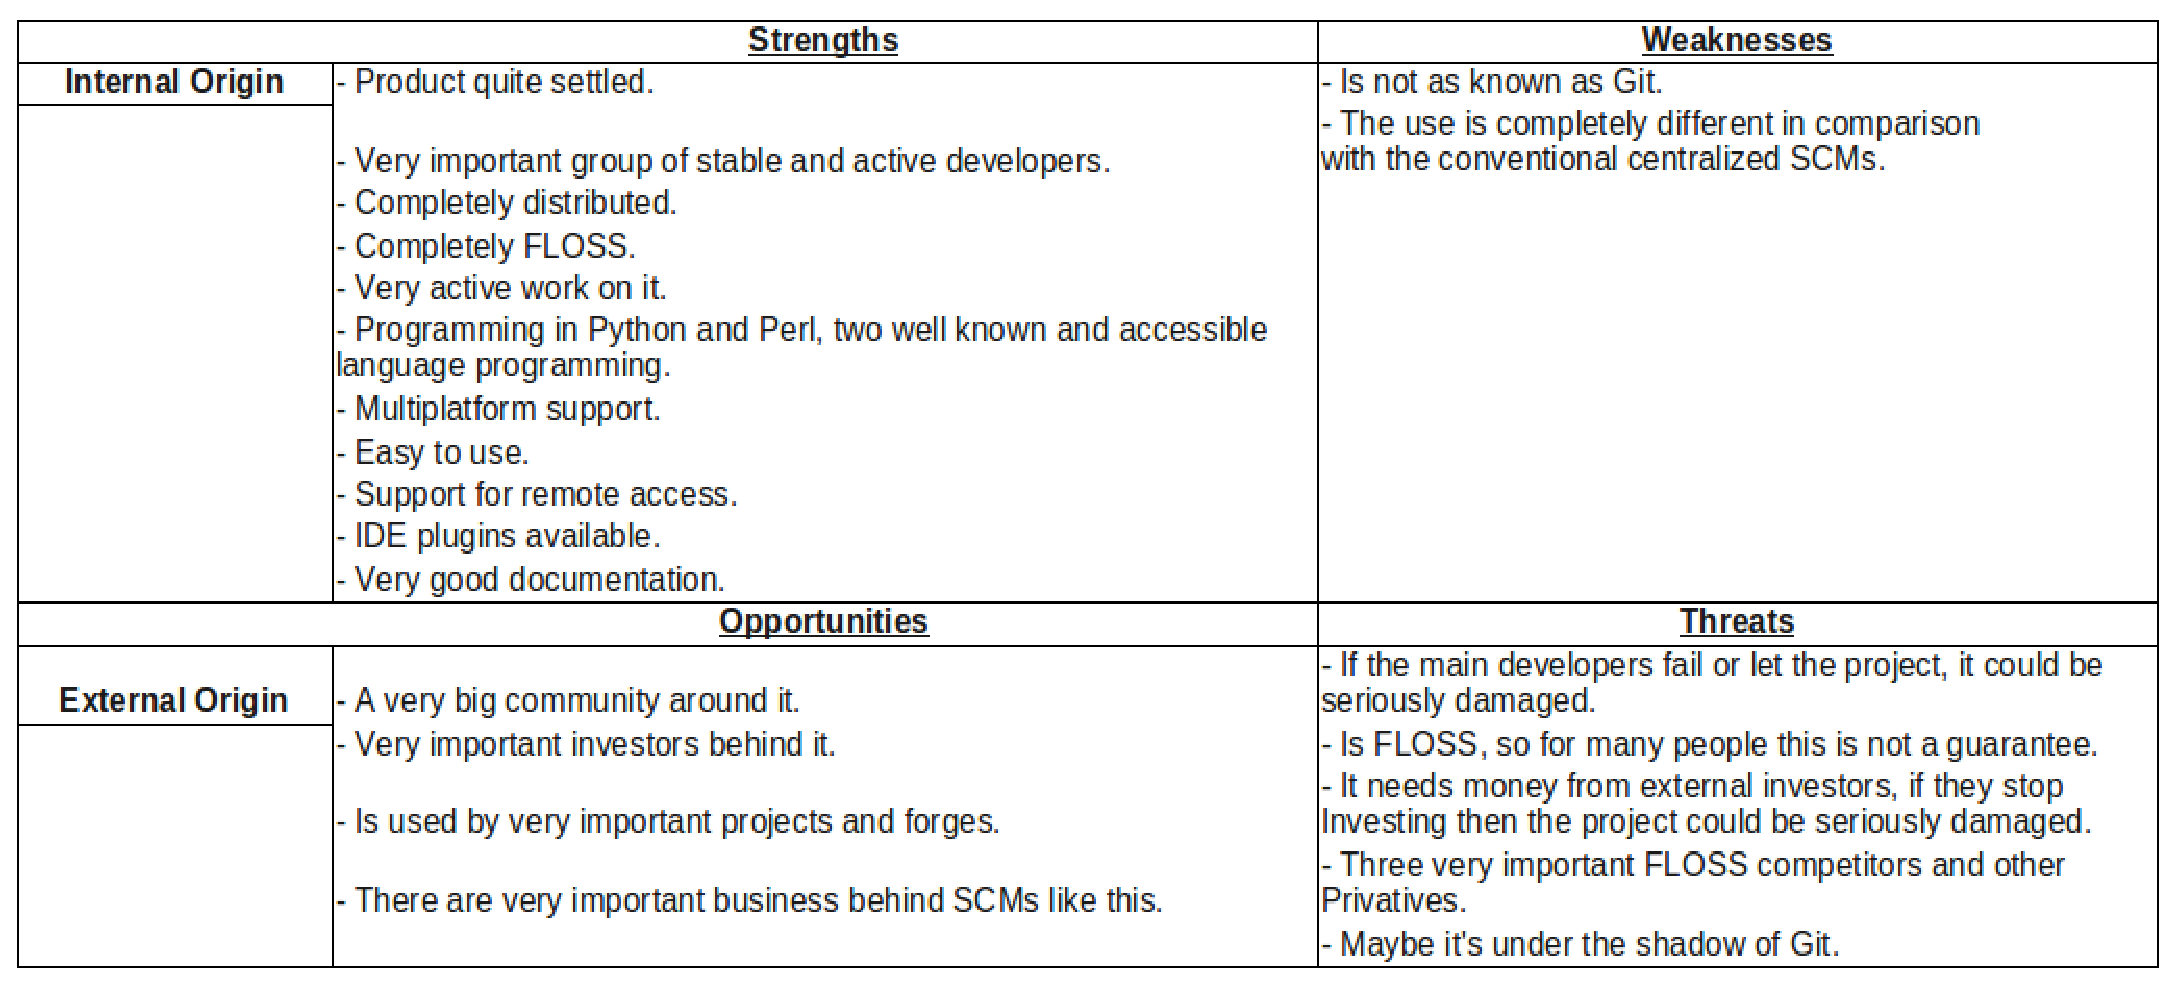
\includegraphics[width=15cm, keepaspectratio]{img/swot_analysis.pdf}
    \caption{\textit{SWOT Analysis}}
    \label{figure:swot_analysis}
 \end{figure}

As we can see, there are more good points than bad points, both in
\textit{strengths} and \textit{opportunities} in comparison with
\textit{weaknesses} and \textit{Threats}.

In fact there are, under our point of view, just two pints which are dangerous
for our project:
\begin{itemize}
 \item The usage is completely different in comparison with distributed SCMs.
 \item The necessity to have investors to maintain the project, economically
talking.
\end{itemize}

\newpage

%%%%%%%%%%%%%%%%%%%%%%%%%%%%%%%%%%%%%%%%%%%%%%%%%%%%%%%%%%%%%%%%%%%%%
\begin{thebibliography}{25}
\bibliographystyle{alpha} 

\bibitem{Android}\textbf{Android}\\
{\footnotesize\url{http://www.android.com/}}

\bibitem{Smartphone}\textbf{Smartphone OS popularity comparison}\\
{\footnotesize\url{http://blog.nielsen.com/nielsenwire/?p=27418}}

\bibitem{Onion}\textbf{“The social structure of Free and Open Source software
development ”, article by Kevin Crowston and James Howison}\\
{\footnotesize\url{
http://docencia.etsit.urjc.es/moodle/mod/resource/view.php?id=4143}}

\bibitem{SCM}\textbf{SCM}\\
{\footnotesize\url{
http://en.wikipedia.org/wiki/Software_configuration_management}}

\bibitem{Subversion}\textbf{Subversion}\\
{\footnotesize\url{http://subversion.tigris.org/}}

\bibitem{Git}\textbf{Git}\\
{\footnotesize\url{http://git-scm.com/}}

\bibitem{Mercurial}\textbf{Mercurial}\\
{\footnotesize\url{http://mercurial.selenic.com/}}

\bibitem{CVS}\textbf{CVS}\\
{\footnotesize\url{http://www.cvshome.org/}}

\bibitem{AndroidPlugin}\textbf{Android Development Tools Plugin}\\
{\footnotesize\url{http://developer.android.com/sdk/eclipse-adt.html}}

\bibitem{Drupal}\textbf{Drupal}\\
{\footnotesize\url{http://drupal.org/}}

\bibitem{GoogleCode}\textbf{Google Code forge}\\
{\footnotesize\url{http://code.google.com/projecthosting/}}

\bibitem{Launchpad}\textbf{Launchpad forge}\\
{\footnotesize\url{https://launchpad.net/}}

\bibitem{Sourceforge}\textbf{Sourceforge forge}\\
{\footnotesize\url{http://sourceforge.net/}}

\bibitem{Github}\textbf{Github forge}\\
{\footnotesize\url{https://github.com/}}

\bibitem{Ohloh}\textbf{Ohloh}\\
{\footnotesize\url{http://www.ohloh.net/}}

\bibitem{FLOSSMetrics}\textbf{FLOSSMetrics}\\
{\footnotesize\url{http://flossmetrics.org/}}

\bibitem{OpenBRRWhitepaper}\textbf{OpenBRR: Business Readiness Rating for
Open Source (White paper)}\\
{\footnotesize\url{
http://docencia.etsit.urjc.es/moodle/mod/resource/view.php?id=4343}}

\bibitem{OpenBRR_amiguetes}\textbf{OpenBRR spreadsheet tailored for Amiguetes
S.L}\\
{\footnotesize\url{
https://gitorious.org/mswl-eval/mswl-eval/blobs/master/ProjectEvaluation_Report/
OpenBRR_Templates/BRR_Template_amiguetes.ods}}


%---- Subversion -------%
\bibitem{Subversion (Wikipedia)}\textbf{Subversion (Wikipedia)}\\
{\footnotesize\url{https://en.wikipedia.org/wiki/Apache_Subversion}}

\bibitem{FSFS}\textbf{FSFS}\\
{\footnotesize\url{
http://svnbook.red-bean.com/en/1.7/svn.reposadmin.planning.html#svn.reposadmin.b
asics.backends
}}

\bibitem{Apache}\textbf{Subversion joins the ASF}\\
{\footnotesize\url{http://www.open.collab.net/news/press/2009/svn-asf.html}}

\bibitem{Wandisco}\textbf{WANdisco hire Subversion core commiters}\\
{\footnotesize\url{
http://www.prweb.com/releases/infrastructure/software/prweb4967504.htm}}

\bibitem{ASFwandisco}\textbf{ASF and WANdisco collaboration}\\
{\footnotesize\url{
https://blogs.apache.org/foundation/entry/apache\_subversion\_to\_wandisco_1}}

\bibitem{Contributors}\textbf{Subversion contributors page}\\
{\footnotesize\url{https://subversion.apache.org/contributing.html}}

\bibitem{SVNreleases}\textbf{Subversion Releases}\\
{\footnotesize\url{
https://subversion.apache.org/docs/community-guide/releasing.html}}

\bibitem{SVNroadmap}\textbf{Subversion Roadmap}\\
{\footnotesize\url{https://subversion.apache.org/roadmap.html}}

\bibitem{APL}\textbf{Apache License compatibility with GPL v3}\\
{\footnotesize\url{http://www.apache.org/licenses/GPL-compatibility.html}}

%---- Mercurial -------%
\bibitem{Mercurial (Wikipedia)}\textbf{Mercurial (Wikipedia)}\\
{\footnotesize\url{http://en.wikipedia.org/wiki/Mercurial}}

\bibitem{3-way merge}\textbf{3-way merge}\\
{\footnotesize\url{http://en.wikipedia.org/wiki/3-way_merge#Three-way_merge}}

\bibitem{swot_analysis}\textbf{SWOT Analysis (Wikipedia)}\\
{\footnotesize\url{http://en.wikipedia.org/wiki/SWOT_analysis}}


\end{thebibliography}
\end{document}
